% Task C16
% Source volume: lower
% Physical scan pages: 118--148
% Printed book pages: 106--136
% Transcribe only source content; omit running headers, footers, and printed page numbers.
\chapter{无穷级数的应用}

无穷级数作为一种分析手段具有多方面的应用，本章只介绍其中的几点供教学中参考。§16.1 是级数在积分计算中的应用。§16.2 讨论级数求和问题。§16.3 是关于 Weierstrass 逼近定理的证明方法及其应用。§16.4 用无穷级数构造一些具有特殊性质的函数。最后一节为学习要点和参考题。

\section{积分计算}

从上册第九章不定积分已经知道，初等函数的原函数未必是初等函数。因此在第十章中用 Newton--Leibniz 公式计算积分的方法的适用范围是有限的。在 12.3.2 小节（见上册 390 页）中列举了几个特殊的广义积分的计算，可以说每一个例题都有其特殊的方法。本节将从方法论的角度介绍无穷级数在积分计算中的应用。这方面的更一般性讨论见后面第二十三章的含参变量积分。

\subsection{关于逐项积分的补充命题}

利用函数项级数的逐项积分法可以计算出许多在定积分或广义积分理论中无法计算的积分。对于常义积分来说，应用一致收敛充分条件下的逐项积分，或者 Arzelà 控制收敛定理（命题 14.2.4）一般就可以解决问题。但是对于广义积分问题则还需要补充几个新的工具。下面只对无穷限广义积分写出保证逐项积分成立的两个命题，它们当然可以推广到有限区间上的瑕积分上去。

\begin{xproposition}[16.1.1]
设在区间 $[a,+\infty)$ 上的连续函数列 $\{f_n\}$ 单调收敛于连续函数 $\varphi$，又设每个 $f_n\ (n=1,2,\ldots)$ 和 $\varphi$ 均在区间 $[a,+\infty)$ 上广义可积，则成立
\[
  \lim_{n\to\infty}\int_a^{+\infty}f_n(x)\,\dd x
  =\int_a^{+\infty}\varphi(x)\,\dd x.
\]
\end{xproposition}

\begin{xproof}
为确定起见，只对连续函数列 $\{f_n\}$ 单调减少的情况写出证明。对于 $A>a$ 写出
\begin{equation}
\begin{aligned}
0&\leqslant \int_a^{+\infty}f_n(x)\,\dd x-\int_a^{+\infty}\varphi(x)\,\dd x\\
 &=\int_a^A[f_n(x)-\varphi(x)]\,\dd x+\int_A^{+\infty}[f_n(x)-\varphi(x)]\,\dd x.
\end{aligned}
\tag{16.1}
\label{eq:16.1}
\end{equation}
利用 $\{f_n\}$ 单调减少收敛于 $\varphi$，取定 $N$，由于 $f_N$ 和 $\varphi$ 在 $[a,+\infty)$ 上均广义可积，因此对于每个给定的 $\varepsilon>0$，可以取定 $A$，使得
\[
  0\leqslant\int_A^{+\infty}[f_N(x)-\varphi(x)]\,\dd x<\varepsilon.
\]
因此当 $n>N$ 时 (16.1) 右边的第二项满足估计：
\[
  0\leqslant\int_A^{+\infty}[f_n(x)-\varphi(x)]\,\dd x
  \leqslant\int_A^{+\infty}[f_N(x)-\varphi(x)]\,\dd x<\varepsilon.
\]
然后在区间 $[a,A]$ 上利用（42 页上的）Dini 定理知道 $\{f_n\}$ 一致收敛于 $\varphi$，因此存在 $N_1>N$，使得当 $n>N_1$ 时 (16.1) 右边的第一项也小于 $\varepsilon$。
\end{xproof}

\begin{xremark}
对于函数项级数有相应的结论，从略。
\end{xremark}

为建立更一般的充分条件，需引入一个新的概念（参见命题 14.2.2 后的说明）。

\begin{xdefinition}
设函数列 $\{f_n\}$ 中的每个函数在区间 $[a,+\infty)$ 上均广义可积，如果对于任意 $\varepsilon>0$，存在 $A_0>a$，使得当 $A>A_0$ 时
\[
  \left|\int_A^{+\infty}f_n(x)\,\dd x\right|<\varepsilon
\]
对于所有 $n$ 同时成立，则称（含参变量 $n$ 的）广义积分 $\int_a^{+\infty}f_n(x)\,\dd x$ 关于 $n$ \textbf{一致收敛}。
\end{xdefinition}

\begin{xproposition}[16.1.2]
设在区间 $[a,+\infty)$ 上函数列 $\{f_n\}$ 内闭一致收敛于函数 $\varphi$，又设 $\{f_n\}\ (n=1,2,\ldots)$ 在区间 $[a,+\infty)$ 上的广义积分关于 $n$ 一致收敛，且极限函数 $\varphi$ 于 $[a,+\infty)$ 上内闭可积，则成立
\[
  \lim_{n\to\infty}\int_a^{+\infty}f_n(x)\,\dd x
  =\int_a^{+\infty}\varphi(x)\,\dd x.
\]
\end{xproposition}

\begin{xproof}
（只列出主要步骤）先用 Cauchy 收敛准则证明 $\varphi$ 于 $[a,+\infty)$ 上广义可积，然后可用三分法估计如下：
\[
\begin{aligned}
\left|\int_a^{+\infty}f_n(x)\,\dd x-\int_a^{+\infty}\varphi(x)\,\dd x\right|
&\leqslant\left|\int_a^A[\varphi(x)-f_n(x)]\,\dd x\right|\\
&\quad+\left|\int_A^{+\infty}\varphi(x)\,\dd x\right|
+\left|\int_A^{+\infty}f_n(x)\,\dd x\right|.
\end{aligned}
\]
\end{xproof}

\begin{xremark}
将上两个命题所要建立的等式改写为
\begin{equation}
  \lim_{n\to\infty}\lim_{A\to+\infty}\int_a^A f_n(x)\,\dd x
  =\lim_{A\to+\infty}\lim_{n\to\infty}\int_a^A f_n(x)\,\dd x,
\tag{16.2}
\label{eq:16.2}
\end{equation}
并应用极限顺序交换的基本原理（见命题 14.2.1 后的注以及命题 14.2.2），就可以知道上述命题中的广义积分关于 $n$ 的一致收敛条件可以更换为
\[
  \lim_{n\to\infty}\int_a^A f_n(x)\,\dd x=\int_a^A\varphi(x)\,\dd x
\]
关于 $A\in[a,+\infty)$ 的一致性。
\end{xremark}

\subsection{例题}

首先需指出，这里的要点是将积分计算问题转化为级数求和问题。在这之后的问题从数值角度来说就是近似计算问题。至于是否所求的积分值都有简单的表达式，即能够用熟悉的常数和有限次初等运算得到，那当然不一定。

\begin{xexample}[16.1.1]
出现在一系列应用问题中的积分
\begin{equation}
  E(k)=\int_0^{\pi/2}\sqrt{1-k^2\sin^2\varphi}\,\dd\varphi
\tag{16.3}
\label{eq:16.3}
\end{equation}
称为\textbf{第二类完全椭圆积分}，其中 $k\in(0,1)$ 为参数。试将 $E(k)$ 展开为 $k$ 的幂级数，并利用它研究椭圆周长近似公式
\begin{equation}
  s_1=\frac{\pi}{2}\left[a+b+\sqrt{2a^2+2b^2}\right]
\tag{16.4}
\label{eq:16.4}
\end{equation}
当椭圆偏心率充分小时的误差的渐近性态，其中 $a>b>0$ 为椭圆的长半轴和短半轴，偏心率 $\varepsilon=\sqrt{a^2-b^2}/a$。（公式 (16.4) 来自上册 356 页的例题 11.3.3。）
\end{xexample}

\begin{xsolution}
除了 $k=0,1$ 之外，积分 (16.3) 的被积函数没有初等原函数（参见上册 297 页），但要将 $E(k)$ 展开为幂级数则是容易的。在 $(1-x)^{1/2}$ 的 Maclaurin 级数中令 $x=k^2\sin^2\varphi$ 代入，就得到
\[
  (1-k^2\sin^2\varphi)^{1/2}
  =1-\sum_{n=1}^{\infty}\frac{(2n-3)!!}{2^n n!}k^{2n}\sin^{2n}\varphi,
  \qquad 0\leqslant k<1.
\]
以 $k$ 为参数，以 $\varphi\in[0,\pi/2]$ 为自变量，这是同号函数项级数，从 Dini 定理可知一致收敛，因此可以逐项积分，这样就得到所要的展开式：
\[
  E(k)=\frac{\pi}{2}\left(1-\sum_{n=1}^{\infty}
  \left[\frac{(2n-1)!!}{(2n)!!}\right]^2\frac{k^{2n}}{2n-1}\right).
\]
椭圆周长可以表示为
\[
  s=4a\int_0^{\pi/2}\sqrt{1-\varepsilon^2\sin^2\varphi}\,\dd\varphi
  =4aE(\varepsilon),\qquad 0<\varepsilon<1,
\]
因此就有
\begin{equation}
\begin{aligned}
  s=2\pi a\biggl(&1-\frac14\varepsilon^2-\frac{3}{64}\varepsilon^4
  -\frac{5}{256}\varepsilon^6-\frac{175}{16\,384}\varepsilon^8\\
  &-\frac{441}{65\,536}\varepsilon^{10}-\frac{4\,851}{1\,048\,576}\varepsilon^{12}\biggr)
  +\bigO(\varepsilon^{14})\qquad(\varepsilon\to0).
\end{aligned}
\tag{16.5}
\label{eq:16.5}
\end{equation}
同时将近似计算公式 (16.4) 右边按 $\varepsilon$ 展开，并与上式比较得到：
\[
  s_1=s-2\pi a\cdot\frac{5}{16\,384}\varepsilon^8+\bigO(\varepsilon^{10})
  \qquad(\varepsilon\to0).
\]
\end{xsolution}

\begin{xremark}
本题取材于 [44] 卷 2 第八章 §7，其中还有椭圆周长的另一个近似公式
\begin{equation}
  s_2=\pi\left[\frac32(a+b)-\sqrt{ab}\right].
\tag{16.6}
\label{eq:16.6}
\end{equation}
采用同样的分析方法可以知道
\[
  s_2=s+2\pi a\cdot\frac{3}{16\,384}\varepsilon^8+\bigO(\varepsilon^{10})
  \qquad(\varepsilon\to0).
\]
容易看出，这两个公式的误差符号相反，若采取加权平均的方法就可能得到更好的结果：将 (16.4) 乘 $3/8$ 与 (16.6) 乘 $5/8$ 再相加，就得到新公式：
\begin{equation}
  s_3=\pi\left[\frac98(a+b)+\frac{3}{16}\sqrt{2a^2+2b^2}-\frac58\sqrt{ab}\right].
\tag{16.7}
\label{eq:16.7}
\end{equation}
可以发现新公式的幂级数展开式的 $\varepsilon^8$ 项和 $\varepsilon^{10}$ 项的系数与 (16.5) 的展开式完全相同。这里前者是预期的，而后者是意外的。于是误差的级别为 $\bigO(\varepsilon^{12})$：
\[
  s_3=s-2\pi a\cdot\frac{7}{1\,048\,576}\varepsilon^{12}+\bigO(\varepsilon^{14}).
\]
从数值计算可以知道，这个近似公式不仅在 $\varepsilon$ 充分小时有效，而且直到 $\varepsilon=0.9$ 时的相对误差还小于 $10^{-4}$。
\end{xremark}

利用极限顺序交换的方法可以较简单地计算上册的命题 12.3.7 中的 Euler--Poisson 积分（即概率积分）。

\begin{xexample}[16.1.2]
利用
\[
  \lim_{n\to\infty}\left(1+\frac{x^2}{n}\right)^{-n}=\ee^{-x^2}
\]
证明：
\[
  \int_0^{+\infty}\ee^{-x^2}\,\dd x=\frac{\sqrt\pi}{2}.
\]
\end{xexample}

\begin{xsolution}
用平均值不等式可以看出
\[
  \left(1+\frac{x^2}{n}\right)^n
  =1\cdot\left(1+\frac{x^2}{n}\right)^n
  \leqslant\left[\frac{1+n(1+x^2/n)}{n+1}\right]^{n+1}
  =\left(1+\frac{x^2}{n+1}\right)^{n+1},
\]
因此在区间 $[0,+\infty)$ 上函数列
$\left\{(1+x^2/n)^{-n}\right\}$ 单调减少收敛于极限函数 $\ee^{-x^2}$。应用命题 16.1.1 即有
\[
  \lim_{n\to\infty}\int_0^{+\infty}\left(1+\frac{x^2}{n}\right)^{-n}\,\dd x
  =\int_0^{+\infty}\ee^{-x^2}\,\dd x.
\]
用变量替换 $x=\sqrt n\tan t$ 计算左边极限号下的积分如下：
\[
\begin{aligned}
  \int_0^{+\infty}\left(1+\frac{x^2}{n}\right)^{-n}\,\dd x
  &=\sqrt n\int_0^{\pi/2}\cos^{2n-2}t\,\dd t\\
  &=\frac{\sqrt{n\pi}}2\cdot\frac{(2n-3)!!}{(2n-2)!!}
  \sim\frac{\sqrt{n\pi}}2\cdot\frac1{\sqrt{n\pi}}
  =\frac{\sqrt\pi}{2},
\end{aligned}
\]
这里最后一步利用了 Wallis 公式 (11.29)。
\end{xsolution}

\begin{xexample}[16.1.3]
（Euler 积分）证明：若 $0<p<1$，则
\[
  \int_0^{+\infty}\frac{\dd x}{x^p(1+x)}=\frac{\pi}{\sin\pi p}.
\]
\end{xexample}

\begin{xproof}
将积分拆开为区间 $[0,1]$ 和 $[1,+\infty)$ 上的两个积分。

在区间 $(0,1)$ 上
\[
  \frac1{x^p(1+x)}=\sum_{n=0}^{\infty}(-1)^n x^{n-p},
\]
它在 $(0,1)$ 上虽然不一致收敛，但除去第一项之外，级数的部分和在 $[0,1]$ 上一致有界，因此可以根据 Arzelà 定理（即命题 14.2.4）交换积分与求和的顺序\footnote{若不用 Arzelà 定理，则可以用 14.2.4 小节的题 5。}，得到
\[
\begin{aligned}
  \int_0^1\frac{\dd x}{x^p(1+x)}
  &=\int_0^1\left(\frac1{x^p}+\sum_{n=1}^{\infty}(-1)^n x^{n-p}\right)\dd x\\
  &=\frac1{1-p}+\sum_{n=1}^{\infty}(-1)^n\int_0^1x^{n-p}\,\dd x\\
  &=\frac1{1-p}+\sum_{n=1}^{\infty}\frac{(-1)^n}{n+1-p}
  =\sum_{n=1}^{\infty}\frac{(-1)^{n-1}}{n-p}.
\end{aligned}
\]
对于 $[1,+\infty)$ 上的积分可作变量替换变为 $[0,1]$ 上的积分，经同样计算得到
\[
\begin{aligned}
  \int_1^{+\infty}\frac{\dd x}{x^p(1+x)}
  &=\int_0^1\frac{\dd x}{x^{1-p}(1+x)}\\
  &=\sum_{n=1}^{\infty}\frac{(-1)^{n-1}}{n-(1-p)}
  =\frac1p+\sum_{n=1}^{\infty}\frac{(-1)^n}{n+p}.
\end{aligned}
\]
合并两个结果得到
\[
\begin{aligned}
  \int_0^{+\infty}\frac{\dd x}{x^p(1+x)}
  &=\frac1p+\sum_{n=1}^{\infty}(-1)^n\left(\frac1{p-n}+\frac1{p+n}\right)\\
  &=\frac1p+\sum_{n=1}^{\infty}(-1)^n\frac{2p}{p^2-n^2}.
\end{aligned}
\]
最后利用余割函数 $\csc x$ 的部分分式展开式就得到所求结果。（该公式见 15.2.7 小节练习题 3，也可以从 $\sin x$ 的无穷乘积展开式 (13.30) 求导得到。）
\end{xproof}

\begin{xremark}
本题的积分有各种不同的形式，例如
\[
  \int_0^{+\infty}\frac{x^{a-1}\,\dd x}{1+x}\quad(0<a<1),\qquad
  \int_0^{+\infty}\frac{x^{m-1}\,\dd x}{1+x^n}\quad(0<m<n)
\]
等。此外，上册 402 页题 8 中的所有公式均为本题之特例，且其中的参数 $m,n$ 等都可以不限于正整数。读者可以对比两处所用方法，从而知道在积分计算问题中我们已经取得的进步。
\end{xremark}

在上册 400 页的题 16 引进了 $x>0$ 时的 $\Gamma$ 函数的积分定义，在例题 13.4.4 中又引进了它的无穷乘积定义。利用积分号下取极限的过程，我们可以证明当 $x>0$ 时两个定义是一致的。

\begin{xexample}[16.1.4]
当 $x>0$ 时成立
\[
  \Gamma(x)=\int_0^{+\infty}t^{x-1}\ee^{-t}\,\dd t
  =\lim_{n\to\infty}\frac{n!n^x}{x(x+1)\cdots(x+n)}.
\]
\end{xexample}

\begin{xproof}
在广义积分中作变量替换 $t=\ln(1/s)$，当 $t$ 从 $0$ 到 $+\infty$ 时，$s$ 从 $1$ 到 $0$，于是得到
\[
  \Gamma(x)=\int_0^1\left(\ln\frac1s\right)^{x-1}\,\dd s.
\]
利用
\[
  \ln\frac1s=\lim_{n\to\infty}n(1-s^{1/n}),
\]
而且右边的极限过程关于 $n$ 单调，就可以用命题 16.1.1 得到
\[
  \Gamma(x)=\lim_{n\to\infty}\int_0^1\left[n(1-s^{1/n})\right]^{x-1}\,\dd s.
\]
对于右边的积分用变量替换 $s^{1/n}=y$，然后多次分部积分即可。
\end{xproof}

\subsection{练习题}

\begin{xexercise}[1]
（广义积分的控制收敛定理）设函数列 $\{S_n(x)\}$ 在 $(-\infty,+\infty)$ 上内闭可积，且内闭一致收敛于函数 $S$，如果存在函数 $F$，使 $|S_n(x)|\leqslant F(x)$ 对于每个 $n$ 和每个 $x$ 都成立，且广义积分 $\int_{-\infty}^{+\infty}F(x)\,\dd x$ 收敛，证明：
\[
  \lim_{n\to\infty}\int_{-\infty}^{+\infty}S_n(x)\,\dd x
  =\int_{-\infty}^{+\infty}S(x)\,\dd x.
\]
\end{xexercise}
\begin{xsolution}
由内闭一致收敛，逐点有 $S_n(x)\to S(x)$。又由 $|S_n(x)|\leqslant F(x)$ 取极限得
\[
  |S(x)|\leqslant F(x).
\]
因为 $F$ 在 $(-\infty,+\infty)$ 上广义可积，所以 $S$ 也广义可积。

任取 $\varepsilon>0$。由 $F$ 的广义积分收敛，可取 $A>0$，使得
\[
  \int_{(-\infty,-A]\cup[A,+\infty)}F(x)\,\dd x<\varepsilon.
\]
于是在两端尾部有
\[
\begin{aligned}
  \left|\int_{(-\infty,-A]\cup[A,+\infty)}S_n(x)\,\dd x\right|&<\varepsilon,\\
  \left|\int_{(-\infty,-A]\cup[A,+\infty)}S(x)\,\dd x\right|&<\varepsilon.
\end{aligned}
\]
在闭区间 $[-A,A]$ 上，$S_n\to S$ 一致，因此存在 $N$，使 $n\geqslant N$ 时
\[
  \sup_{|x|\leqslant A}|S_n(x)-S(x)|<\frac{\varepsilon}{2A+1}.
\]
从而
\[
  \left|\int_{-A}^A[S_n(x)-S(x)]\,\dd x\right|<\varepsilon.
\]
合并中间区间和两端尾部，得
\[
  \left|\int_{-\infty}^{+\infty}S_n(x)\,\dd x-
  \int_{-\infty}^{+\infty}S(x)\,\dd x\right|<3\varepsilon.
\]
故
\[
  \lim_{n\to\infty}\int_{-\infty}^{+\infty}S_n(x)\,\dd x
  =\int_{-\infty}^{+\infty}S(x)\,\dd x.
\]
\end{xsolution}


\begin{xexercise}[2]
设 $\sum_{n=0}^{\infty}a_nx^n$ 的系数均非负，收敛半径为 $+\infty$，和函数为 $S(x)$。证明：如果 $\sum_{n=0}^{\infty}a_nn!$ 收敛，则广义积分 $\int_0^{+\infty}\ee^{-x}S(x)\,\dd x$ 也收敛，且等于 $\sum_{n=0}^{\infty}a_nn!$。

（去掉系数非负条件后本题结论仍成立，这时可以利用命题 16.1.2 后的注。）
\end{xexercise}
\begin{xsolution}
记
\[
  S_N(x)=\sum_{n=0}^N a_nx^n.
\]
由于 $a_n\geqslant0$，对 $x\geqslant0$ 有 $S_N(x)\uparrow S(x)$。对每个 $N$，逐项积分得到
\[
\begin{aligned}
  \int_0^{+\infty}\ee^{-x}S_N(x)\,\dd x
  &=\sum_{n=0}^Na_n\int_0^{+\infty}x^n\ee^{-x}\,\dd x\\
  &=\sum_{n=0}^Na_nn!.
\end{aligned}
\]
设 $L=\sum_{n=0}^{\infty}a_nn!<+\infty$。对任意 $A>0$，幂级数在 $[0,A]$ 上一致收敛，故
\[
  \int_0^A\ee^{-x}S(x)\,\dd x
  =\lim_{N\to\infty}\int_0^A\ee^{-x}S_N(x)\,\dd x
  \leqslant L.
\]
左边关于 $A$ 单调增加且有上界 $L$，所以广义积分收敛。另一方面，对每个 $N$，
\[
  \int_0^{+\infty}\ee^{-x}S(x)\,\dd x
  \geqslant\int_0^{+\infty}\ee^{-x}S_N(x)\,\dd x
  =\sum_{n=0}^Na_nn!.
\]
令 $N\to\infty$ 得积分不小于 $L$；而前面的估计令 $A\to+\infty$ 又给出积分不大于 $L$。因此
\[
  \int_0^{+\infty}\ee^{-x}S(x)\,\dd x
  =\sum_{n=0}^{\infty}a_nn!.
\]
\end{xsolution}


\begin{xexercise}[3]
证明下列结果：
\begin{enumerate}[label=(\arabic*)]
\item $\displaystyle \int_0^1\frac{\ln(1-x)}x\,\dd x=-\sum_{n=1}^{\infty}\frac1{n^2}$；
\item $\displaystyle \int_0^1\frac{\ln x}{1-x^2}\,\dd x=-\frac{\pi^2}{8}$；
\item $\displaystyle \int_0^1\ln x\ln(1-x)\,\dd x=2-\frac{\pi^2}{6}$；
\item $\displaystyle \int_0^{+\infty}\frac{x}{\ee^x-\ee^{-x}}\,\dd x=\frac{\pi^2}{8}$。
\end{enumerate}
\end{xexercise}
\begin{xsolution}
\textbf{(1)}\quad
对 $0\leqslant x<1$，
\[
  -\ln(1-x)=\sum_{n=1}^{\infty}\frac{x^n}{n}.
\]
各项非负，故可先在 $[0,r]$（$0<r<1$）逐项积分，再令 $r\to1^-$：
\[
\begin{aligned}
  -\int_0^1\frac{\ln(1-x)}x\,\dd x
  &=\sum_{n=1}^{\infty}\frac1n\int_0^1x^{n-1}\,\dd x\\
  &=\sum_{n=1}^{\infty}\frac1{n^2}.
\end{aligned}
\]
于是
\[
  \int_0^1\frac{\ln(1-x)}x\,\dd x
  =-\sum_{n=1}^{\infty}\frac1{n^2}.
\]

\textbf{(2)}\quad
对 $0\leqslant x<1$，
\[
  \frac1{1-x^2}=\sum_{n=0}^{\infty}x^{2n}.
\]
又
\[
  \int_0^1x^{\alpha}\ln x\,\dd x=-\frac1{(\alpha+1)^2}\qquad(\alpha>-1).
\]
把负号提出后，
\[
  \frac{-\ln x}{1-x^2}=\sum_{n=0}^{\infty}x^{2n}(-\ln x),
  \qquad 0<x<1,
\]
右边各项非负。因此可对非负级数使用单调收敛（等价地，先在 $[0,r]$ 上逐项积分再令 $r\to1^-$），得到
\[
  \int_0^1\frac{\ln x}{1-x^2}\,\dd x
  =-\sum_{n=0}^{\infty}\frac1{(2n+1)^2}.
\]
由
\[
  \sum_{n=0}^{\infty}\frac1{(2n+1)^2}
  =\left(1-\frac14\right)\sum_{n=1}^{\infty}\frac1{n^2}
  =\frac{\pi^2}{8},
\]
故
\[
  \int_0^1\frac{\ln x}{1-x^2}\,\dd x=-\frac{\pi^2}{8}.
\]

\textbf{(3)}\quad
由
\[
  -\ln(1-x)=\sum_{n=1}^{\infty}\frac{x^n}{n}
\]
和各项非负性，
\[
\begin{aligned}
  \int_0^1\ln x\ln(1-x)\,\dd x
  &=\sum_{n=1}^{\infty}\frac1n\int_0^1(-\ln x)x^n\,\dd x\\
  &=\sum_{n=1}^{\infty}\frac1{n(n+1)^2}.
\end{aligned}
\]
分解
\[
  \frac1{n(n+1)^2}=\frac1n-\frac1{n+1}-\frac1{(n+1)^2},
\]
故
\[
\begin{aligned}
  \sum_{n=1}^{\infty}\frac1{n(n+1)^2}
  &=1-\sum_{n=1}^{\infty}\frac1{(n+1)^2}\\
  &=1-\left(\frac{\pi^2}{6}-1\right)
  =2-\frac{\pi^2}{6}.
\end{aligned}
\]

\textbf{(4)}\quad
当 $x>0$ 时
\[
  \frac{x}{\ee^x-\ee^{-x}}
  =\frac{x\ee^{-x}}{1-\ee^{-2x}}
  =\sum_{n=0}^{\infty}x\ee^{-(2n+1)x},
\]
右边各项非负。于是
\[
\begin{aligned}
  \int_0^{+\infty}\frac{x}{\ee^x-\ee^{-x}}\,\dd x
  &=\sum_{n=0}^{\infty}\int_0^{+\infty}x\ee^{-(2n+1)x}\,\dd x\\
  &=\sum_{n=0}^{\infty}\frac1{(2n+1)^2}
  =\frac{\pi^2}{8}.
\end{aligned}
\]
\end{xsolution}


\begin{xexercise}[4]
证明：$\displaystyle \int_0^1x^{-x}\,\dd x=\sum_{n=1}^{\infty}n^{-n}$。
\end{xexercise}
\begin{xsolution}
对 $0<x\leqslant1$，
\[
  x^{-x}=\ee^{-x\ln x}
  =\sum_{n=0}^{\infty}\frac{x^n(-\ln x)^n}{n!},
\]
各项非负，因此可以逐项积分。利用
\[
  \int_0^1x^n(-\ln x)^n\,\dd x
  =\frac{n!}{(n+1)^{n+1}},
\]
得到
\[
\begin{aligned}
  \int_0^1x^{-x}\,\dd x
  &=\sum_{n=0}^{\infty}\frac1{n!}
    \int_0^1x^n(-\ln x)^n\,\dd x\\
  &=\sum_{n=0}^{\infty}\frac1{(n+1)^{n+1}}
  =\sum_{m=1}^{\infty}m^{-m}.
\end{aligned}
\]
\end{xsolution}


\begin{xexercise}[5]
证明：
\[
  \int_0^{+\infty}x\ee^{-x^2/2}
  \left(1+\frac{x^2}{2^2}+\frac{x^4}{2^2 4^2}+\cdots
  +\frac{x^{2n}}{[(2n)!!]^2}+\cdots\right)\dd x=\ee^{1/2}.
\]
\end{xexercise}
\begin{xsolution}
注意 $(2n)!!=2^nn!$。作变量替换 $y=x^2/2$，则 $x\,\dd x=\dd y$，且
\[
  \frac{x^{2n}}{[(2n)!!]^2}
  =\frac{y^n}{2^n(n!)^2}.
\]
被积级数各项非负，故可逐项积分：
\[
\begin{aligned}
&\int_0^{+\infty}x\ee^{-x^2/2}
  \left(1+\frac{x^2}{2^2}+\frac{x^4}{2^24^2}+\cdots\right)\dd x\\
&\qquad=\sum_{n=0}^{\infty}\frac1{2^n(n!)^2}
  \int_0^{+\infty}y^n\ee^{-y}\,\dd y\\
&\qquad=\sum_{n=0}^{\infty}\frac1{2^nn!}
  =\ee^{1/2}.
\end{aligned}
\]
\end{xsolution}


\section{级数求和计算}

本节列举了级数求和的各种方法供读者参考。其中级数和的概念是在通常意义下的。关于 Cesàro 求和概念见 15.2.3 小节，本节不再讨论。

\subsection{级数求和法}

对于收敛级数来说，原则上已经可以通过数值计算来得到级数和的近似值。但如果能够发现某个级数和（的准确答案）可以用已知常数经过简单运算得到，则当然更好。由 Euler 解决的 Basel 问题，即求出
\[
  1+\frac14+\frac19+\cdots+\frac1{n^2}+\cdots=\frac{\pi^2}{6},
\]
就是级数求和方面的一个光辉例子。在得到这个答案之前，Euler 已经计算出级数和的近似值 $1.644934\ldots$ 直到 20 位有效数字，但仍然看不出级数和是什么特殊的常数。当然没有人想到这里会出现圆周率（参见例题 13.4.3 后的注 3 以及 [16] 的第 3 章）。

从上册命题 2.5.2 中的例子
\[
  \ee=1+1+\frac1{2!}+\cdots+\frac1{n!}+\cdots
\]
可以知道，一个收敛的数项级数（或函数项级数）的和（或和函数）未必能够用过去已经掌握的数或函数经过简单的运算表示出来。例如，直到现在为止对于 $p$ 级数的和
\[
  \zeta(p)=1+\frac1{2^p}+\cdots+\frac1{n^p}+\cdots,
\]
当 $p$ 为奇数时是否会与 $p$ 为偶数时 Euler 的结果（见上册 217 页 (7.26) 和下面的例题 16.2.3）有类似的表达式，始终还只是一个猜测。目前最好的结果是在 1978 年 Apéry（阿佩里）证明了 $\zeta(3)$ 为无理数（见《美国数学月刊》(2001) 第 108 卷 222--231 页）。

因此，在本节只是根据经验列出求级数和的若干方法，这里不可能有什么万能的方法。

\textbf{方法一}\quad 以已知的数项级数或函数项级数展开式为基础的方法无疑是有用的。例如，在一个幂级数展开式或 Fourier 级数展开式中，将变量用不同的特定值代入，就可以得到无穷多个数项级数的和，或者用简单运算将所要研究的级数变换为已知级数等等。当然这完全依赖于积累和经验。

\textbf{方法二}\quad 如果能利用所谓\textbf{裂项相消法}（或连锁消去法）得到部分和的紧凑形式，则级数问题就转化为数列或函数列的极限问题（参见上册 2.2.4 小节的题 3）。

\textbf{方法三}\quad 这也可以看成是方法一的范围，即用函数项级数的逐项积分或逐项微分方法将未知的级数转变为已知的级数。这在幂级数中是最常用的方法，但也可能解决其他类型的函数项级数求和计算。

\textbf{方法四（Abel 方法）}\quad 这是以幂级数理论中的 Abel 第二定理为基础的级数求和方法：对于给定的收敛级数 $\sum_{n=1}^{\infty}a_n$，研究幂级数 $\sum_{n=1}^{\infty}a_nx^n$，它的收敛半径不会小于 1。如果能够求出它的和函数 $S(x)$，则所求的
\[
  S=\sum_{n=1}^{\infty}a_n=\lim_{x\to1^-}S(x)=S(1).
\]

\subsection{例题}

\begin{xexample}[16.2.1]
求下列级数的和：
\[
  \frac{1!}{x+1}+\frac{2!}{(x+1)(x+2)}+\cdots
  +\frac{n!}{(x+1)(x+2)\cdots(x+n)}+\cdots.
\]
\end{xexample}

\begin{xsolution}
\textbf{解 1（裂项相消法）}\quad 易见 $x=1$ 时级数发散。对于 $x\ne1$ 记级数通项为 $a_n$，从前后两项之间的关系式
\[
  a_n(n+x)=na_{n-1}\qquad(a_0=1)
\]
出发得到
\[
  (n+1)a_n+(x-1)a_n=na_{n-1},
\]
可见于 $x\ne1$ 时有
\[
  a_n=\frac1{x-1}[na_{n-1}-(n+1)a_n],
\]
从而可以得到级数的第 $n$ 个部分和为
\[
  S_n=\frac1{x-1}-\frac{(n+1)!}{(x-1)(x+1)\cdots(x+n)},
  \qquad n=1,2,\ldots.
\]
因此问题归结为上式右边第二项的敛散性。利用 Sapagof 判别法（命题 13.2.3）或渐近公式 (13.24) 知第二项当 $x<1$ 时发散，而当 $x>1$ 时收敛于 0。因此级数当 $x\leqslant1$ 时发散，而当 $x>1$ 时收敛于和 $1/(x-1)$。

\begin{xremark}
用裂项相消法求和时一般不必先讨论级数的敛散性。若要讨论本题中的级数的敛散性，则用渐近公式 (13.24) 即可。当然也可用 Raabe 判别法。
\end{xremark}

\textbf{解 2（逐项积分法）}\quad 由敛散性讨论可知只要研究 $x>1$ 的情况。级数的通项（差一个因子 $x$）可以写为积分形式：
\[
  \frac{n!}{x(x+1)\cdots(x+n)}=\int_0^1(1-t)^{x-1}t^n\,\dd t.
\]
（这里虽然 $x$ 未必为正整数，但上册 326 页的分部积分计算仍有效。实际上这都是 23.3.1 小节中 Beta 函数的特例。）用逐项积分法计算如下：
\[
\begin{aligned}
  S(x)&=x\int_0^1\sum_{n=1}^{\infty}(1-t)^{x-1}t^n\,\dd t
      =x\int_0^1(1-t)^{x-2}t\,\dd t\\
  &=\frac{x}{x-1}\int_0^1(1-t)^{x-1}\,\dd t
      =\frac1{x-1}.
\end{aligned}
\]
其中逐项积分的合法性当 $x\geqslant2$ 时可以用 Dini 定理知积分号下的函数项级数 $\sum_{n=1}^{\infty}(1-t)^{x-1}t^n$ 一致收敛来解决，但是当 $1<x<2$ 时 $\int_0^1(1-t)^{x-2}t\,\dd t$ 为收敛的瑕积分，因此需要用命题 16.1.1 的结论。
\end{xsolution}

\begin{xexample}[16.2.2]
（Euler）求级数
\[
  1+\frac14+\frac19+\cdots+\frac1{n^2}+\cdots
\]
的和。
\end{xexample}

这就是历史上的 Basel 问题 [16,17]。Euler 是求出本题答案的第一人。他根据类比猜测出正弦函数的无穷乘积展开式 (13.24)，将它改写为
\[
  \frac{\sin x}{x}=\left(1-\frac{x^2}{\pi^2}\right)
  \left(1-\frac{x^2}{2^2\pi^2}\right)\cdots
  \left(1-\frac{x^2}{n^2\pi^2}\right)\cdots,
\]
其中左边当 $x=0$ 时理解为其极限值 1，因此左边为
\[
  1-\frac{x^2}{6}+\bigO(x^4)\qquad(x\to0).
\]
Euler 又将展开式和多项式的根与系数关系作类比，看出右边应该是
\[
  1-\frac{x^2}{\pi^2}\sum_{n=1}^{\infty}\frac1{n^2}+\bigO(x^4)\qquad(x\to0),
\]
比较两边的 $x^2$ 项的系数就知道所求的级数和为 $\pi^2/6$。下面我们将 Euler 的方法严格化，作为第一个解。

\begin{xsolution}
\textbf{解 1}\quad 在 $\sin x/x$ 的上述无穷乘积展开式中令 $y=x^2/\pi^2$，然后讨论函数
\begin{equation}
  F(y)=\prod_{n=1}^{\infty}\left(1-\frac{y}{n^2}\right).
\tag{16.8}
\label{eq:16.8}
\end{equation}
这时由于 $F(y)=1-y\pi^2/6+\bigO(y^2)\ (y\to0)$，因此只需要从 (16.8) 右边的无穷乘积出发证明函数 $F$ 在 $y=0$ 处的导数 $F'(0)=-\sum_{n=1}^{\infty}1/n^2$ 即可。

对函数 $F$ 在 $|y|<1$ 范围内取对数，并求导得到
\[
  \frac{F'(y)}{F(y)}
  =\sum_{n=1}^{\infty}\frac{-1/n^2}{1-y/n^2}
  =-\sum_{n=1}^{\infty}\frac1{n^2-y},
\]
其中右边逐项求导的合理性容易从 Weierstrass 一致收敛性判别法得到验证，同时这也保证了 $F$ 的可微性。然后令 $y=0$ 代入，利用 $F(0)=1$，可见所求结果成立。因此有
\[
  F(y)=1-y\sum_{n=1}^{\infty}\frac1{n^2}+\littleo(y)\qquad(y\to0),
\]
这样就知道有
\[
  \prod_{n=1}^{\infty}\left(1-\frac{x^2}{n^2\pi^2}\right)
  =1-\frac{x^2}{\pi^2}\sum_{n=1}^{\infty}\frac1{n^2}+\littleo(x^2)\qquad(x\to0),
\]
因此 Euler 的方法是正确的。

\begin{xremark}
在作代换 $y=x^2/\pi^2$ 时有 $y\geqslant0$，但从 (16.8) 可见，$F$ 对于 $y<0$ 仍有意义，因此上述计算是正确的。有兴趣的读者可以用 Euler 公式 $\ee^{\ii\theta}=\cos\theta+\ii\sin\theta$ 对此作出解释。
\end{xremark}

\textbf{解 2（用反正弦函数的幂级数展开式）}\quad 先证明
\begin{equation}
  \sum_{n=1}^{\infty}\frac1{(2n-1)^2}=\frac{\pi^2}{8}.
\tag{16.9}
\label{eq:16.9}
\end{equation}
写出函数 $\arcsin x$ 在 $[-1,1]$ 的幂级数展开式
\[
  \arcsin x=x+\sum_{n=1}^{\infty}\frac{(2n-1)!!}{(2n)!!}\frac{x^{2n+1}}{2n+1},
\]
在其中令 $x=\sin t$，得到
\[
  t=\sin t+\sum_{n=1}^{\infty}
  \frac{(2n-1)!!}{(2n+1)(2n)!!}\sin^{2n+1}t,
  \qquad -\frac\pi2\leqslant t\leqslant\frac\pi2.
\]
将上式两端对 $t$ 从 0 到 $\pi/2$ 积分，并对右端逐项积分，得到
\[
\begin{aligned}
  \frac{\pi^2}{8}
  &=1+\sum_{n=1}^{\infty}\frac{(2n-1)!!}{(2n+1)(2n)!!}
      \int_0^{\pi/2}\sin^{2n+1}t\,\dd t\\
  &=1+\sum_{n=1}^{\infty}\frac{(2n-1)!!}{(2n+1)(2n)!!}
      \cdot\frac{(2n)!!}{(2n+1)!!}\\
  &=1+\sum_{n=1}^{\infty}\frac1{(2n+1)^2}
   =\sum_{n=1}^{\infty}\frac1{(2n-1)^2}.
\end{aligned}
\]
这就证明了 (16.9)。然后从
\[
  S=\sum_{n=1}^{\infty}\frac1{n^2}
   =\sum_{n=1}^{\infty}\frac1{(2n-1)^2}
    +\sum_{n=1}^{\infty}\frac1{(2n)^2}
   =\frac{\pi^2}{8}+\frac S4
\]
即可解出 $S=\pi^2/6$。
\end{xsolution}

\begin{xremark}
\textbf{注 1}\quad 解 2 也是 Euler 找到的，发表于 1743 年（参见 [16]，又见于《美国数学月刊》(1987) 第 94 卷 662--663 页和该刊 (1988) 第 95 卷 331 页。实际上这个思路也出现在 [40] 的第二章的习题 41 中。此外，那里还指出从 $(\arcsin x)^2$ 的 Maclaurin 级数展开式出发也可以达到目的。

\textbf{注 2}\quad 有很多函数的 Fourier 级数展开式可用于此题。例如见例题 15.2.2，这里不再重复。
\end{xremark}

以上的第一种解法可以推广到一般情况，即利用正弦函数的无穷乘积展开式可以求出 $p$ 为偶数时的所有 $p$ 级数之和。这是 Euler 最得意之作。

\begin{xexample}[16.2.3]
证明：对于所有正整数 $n$，$p=2n$ 的 $p$ 级数之和为
\begin{equation}
  s_{2n}=\sum_{m=1}^{\infty}\frac1{m^{2n}}
  =\frac{\overline B_n}{2}\cdot\frac{(2\pi)^{2n}}{(2n)!},
\tag{16.10}
\label{eq:16.10}
\end{equation}
其中 $\overline B_n\ (n\geqslant1)$ 为 Bernoulli 数。前七个 Bernoulli 数为
\[
  \overline B_1=\frac16,\quad \overline B_2=\frac1{30},\quad
  \overline B_3=\frac1{42},\quad \overline B_4=\frac1{30},\quad
  \overline B_5=\frac5{66},\quad \overline B_6=\frac{691}{2730},\quad
  \overline B_7=\frac76
\]
（见上册 7.2.3 小节）。
\end{xexample}

\begin{xproof}
从正弦函数的无穷乘积（见例题 13.4.3）
\[
  \sin x=x\left(1-\frac{x^2}{\pi^2}\right)
  \left(1-\frac{x^2}{2^2\pi^2}\right)\cdots
  =x\prod_{n=1}^{\infty}\left(1-\frac{x^2}{n^2\pi^2}\right)
\]
出发，取绝对值后再取对数，将无穷乘积转化为无穷级数：
\[
  \ln|\sin x|=\ln|x|+\sum_{n=1}^{\infty}\ln\left|1-\frac{x^2}{n^2\pi^2}\right|.
\]
对于 $x\ne k\pi\ (k\in\ZZ)$ 的 $x$，在上式两边求导，得到\footnote{公式 (16.11) 已经出现在 15.2.7 小节的练习题 3，即在函数 $\cos px\ (0<p<1,\ x\in[-\pi,\pi])$ 的 Fourier 展开式中令 $x=\pi$ 代入，再将 $p\pi$ 改记为 $x$。}
\begin{equation}
  \cot x=\frac1x+\sum_{n=1}^{\infty}\frac{2x}{x^2-n^2\pi^2}.
\tag{16.11}
\label{eq:16.11}
\end{equation}
这里逐项求导的合理性不难用 Weierstrass 一致收敛性判别法加以验证，从略。然后在 $|x|<\pi$ 时作以下运算：
\[
\begin{aligned}
  x\cot x
  &=1+2\sum_{m=1}^{\infty}\frac{x^2}{x^2-m^2\pi^2}
   =1-2\sum_{m=1}^{\infty}\frac{x^2/(m^2\pi^2)}{1-x^2/(m^2\pi^2)}\\
  &=1-2\sum_{m=1}^{\infty}\sum_{n=1}^{\infty}
      \left(\frac{x^2}{m^2\pi^2}\right)^n
   =1-2\sum_{n=1}^{\infty}\sum_{m=1}^{\infty}
      \left(\frac{x^2}{m^2\pi^2}\right)^n\\
  &=1-2\sum_{n=1}^{\infty}\frac{s_{2n}}{\pi^{2n}}x^{2n},
  \qquad |x|<\pi,
\end{aligned}
\]
其中 $s_{2n}=\sum_{m=1}^{\infty}1/m^{2n}$ 即是 $p=2n$ 时的 $p$ 级数的和（在以上计算中对二重正项级数求和利用了第十三章第一组参考题 9）。

另一方面，从 (14.25) 已经得到公式
\begin{equation}
  x\cot x=1-\sum_{n=1}^{\infty}\frac{\overline B_n2^{2n}}{(2n)!}x^{2n}.
\tag{16.12}
\label{eq:16.12}
\end{equation}
根据幂级数展开式的惟一性（命题 14.4.1）就可以得到所要的结果。
\end{xproof}

\begin{xremark}
由此可得到 Bernoulli 数的几个重要性质。首先是 $\overline B_n=(-1)^{n-1}B_{2n}>0$。其次，容易证明 $1<s_{2n}<2n/(2n-1)$（见例题 13.2.1），因此由 (16.10) 和 Stirling 公式可以得到 Bernoulli 数的渐近公式：
\begin{equation}
  \overline B_n\sim\frac{2(2n)!}{(2\pi)^{2n}}
  \sim4\sqrt{\pi n}\left(\frac{n}{\pi\ee}\right)^{2n}.
\tag{16.13}
\label{eq:16.13}
\end{equation}
这在确定例题 14.4.2 中的几个幂级数的收敛半径时有用。又从
\[
  \sqrt{2\pi n}\left(\frac n\ee\right)^n<n!
  <\sqrt{2\pi n}\left(\frac n\ee\right)^n\ee^{1/(12n)}
\]
（见上册 374 页题 15）可知，用 (16.13) 右边的渐近公式可以对于 Bernoulli 数 $\overline B_n$ 给出相对误差很小的估计。最后，可由此看出在 $n>\pi\ee\approx8.54$ 之后 Bernoulli 数 $\{\overline B_n\}$ 的增长非常快，虽然 $\overline B_7$ 刚超过 1，但 $\overline B_{13}$ 已经大于 $10^6$。
\end{xremark}

下面的前半题已在本书中见过多次。

\begin{xexample}[16.2.4]
\begin{enumerate}[label=(\arabic*)]
\item 求 Leibniz 型级数的和
\[
  S=1-\frac12+\cdots+\frac{(-1)^{n-1}}n+\cdots;
\]
\item 令
\[
  a_n=1-\frac12+\cdots+\frac{(-1)^{n-1}}n-\ln2,
  \qquad n=1,2,\ldots,
\]
求 $\sum_{n=1}^{\infty}a_n$ 的和。
\end{enumerate}
\end{xexample}

\begin{xsolution}
(1) 用 Abel 方法。根据 Abel 第二定理，有 $S=\lim_{x\to1^-}S(x)$，其中
\[
  S(x)=x-\frac{x^2}{2}+\cdots+\frac{(-1)^{n-1}x^n}{n}+\cdots.
\]
对上式右边的幂级数在 $(-1,1)$ 上逐项求导得到
\[
  S'(x)=1-x+\cdots+(-1)^{n-1}x^{n-1}+\cdots=\frac1{1+x},
\]
又利用 $S(0)=0$，因此可以求出
\[
  S(x)=\int_0^x\frac1{1+t}\,\dd t=\ln(1+x),\qquad -1<x<1.
\]
从而得到
\[
  S=\lim_{x\to1^-}\ln(1+x)=\ln2.
\]

(2) 从 (1) 可见 $a_n$ 就是该级数的第 $n$ 个余项（再乘以 $-1$），因此可以得到
\[
  a_n=\int_0^1\frac{(-1)^{n+1}x^n}{1+x}\,\dd x,
\]
再用 $\sum\int=\int\sum$ 即可得到
\[
  \sum_{n=1}^{\infty}a_n=\ln2-\frac12.
\]
\end{xsolution}

\begin{xremark}
过去已经知道 (1) 中的级数和，但主要是通过 Catalan 恒等式（见上册 55 页）将问题转化为求数列
\[
  \left\{\frac1{n+1}+\frac1{n+2}+\cdots+\frac1{2n}\right\}
\]
的极限问题而解决的（见上册例题 11.4.1 的注）。因此过去的这种方法太特殊了，不如本题的 Abel 求和法可以解决不少级数求和问题。
\end{xremark}

Abel 方法也有可能解决某些函数项级数的求和问题。

\begin{xexample}[16.2.5]
求三角级数 $\sum_{n=1}^{\infty}\cos nx/n$ 的和函数\footnote{对于余弦三角级数也有与例题 15.2.3 和 15.2.4 相同的结论（见 [18] 第三卷的 692 小节），因此事先就可以判定本题的和函数绝对可积，而题中的三角级数为其 Fourier 级数。}。
\end{xexample}

\begin{xsolution}
从函数项级数的敛散性判别法可以知道级数在 $x\ne2k\pi\ (k\in\ZZ)$ 时收敛，因此只需求出 $(0,2\pi)$ 上的和函数 $S(x)$。又从内闭一致收敛知 $S(x)$ 连续。

以 $x$ 为参数，另行引入变量 $\alpha\in(-1,1)$，由 Abel 第二定理有
\[
  S(x)=\lim_{\alpha\to1^-}f(\alpha),
\]
其中
\[
  f(\alpha)=\sum_{n=1}^{\infty}\frac{\cos nx}{n}\alpha^n.
\]
为简明起见在 $f(\alpha)$ 中没有指出与参数 $x$ 的依赖关系。在 $(-1,1)$ 上将此幂级数对 $\alpha$ 逐项求导，并用 Euler 公式计算如下：
\[
\begin{aligned}
  f'(\alpha)
  &=\sum_{n=1}^{\infty}\alpha^{n-1}\cos nx
   =\operatorname{Re}\sum_{n=1}^{\infty}\alpha^{n-1}\ee^{\ii nx}\\
  &=\operatorname{Re}\frac{\ee^{\ii x}}{1-\alpha\ee^{\ii x}}
   =\frac{\cos x-\alpha}{1-2\alpha\cos x+\alpha^2}.
\end{aligned}
\]
然后再利用 $f(0)=0$ 求积得到
\[
  f(\alpha)=-\frac12\ln(1-2\alpha\cos x+\alpha^2),\qquad -1<\alpha<1.
\]
最后就有：
\[
  S(x)=\lim_{\alpha\to1^-}f(\alpha)=f(1)
  =-\frac12\ln 2(1-\cos x)
  =-\ln2-\ln\left|\sin\frac x2\right|.
\]
\end{xsolution}

\begin{xremark}
由所得的等式
\[
  \ln\left|\sin\frac x2\right|=-\ln2-\sum_{n=1}^{\infty}\frac{\cos nx}{n}
\]
出发，可以利用命题 16.1.2 逐项积分，或者利用 Fourier 级数的逐项积分定理（命题 15.2.9）得到 Euler 积分（命题 12.3.4）的值：
\[
  \int_0^{\pi/2}\ln\sin x\,\dd x=-\frac\pi2\ln2,
\]
从而对该积分的计算提供了一种级数解法。
\end{xremark}

下面是 1996 年新发现的圆周率公式（BBP 公式）。

\begin{xexample}[16.2.6]
证明：
\begin{equation}
  \pi=\sum_{n=0}^{\infty}\frac1{16^n}
  \left(\frac4{8n+1}-\frac2{8n+4}-\frac1{8n+5}-\frac1{8n+6}\right).
\tag{16.14}
\label{eq:16.14}
\end{equation}
\end{xexample}

\begin{xproof}
利用逐项积分可知在 $k>0$ 和 $0<x<1$ 时成立
\[
\begin{aligned}
  \int_0^x\frac{t^{k-1}}{1-t^8}\,\dd t
  &=\int_0^x(t^{k-1}+t^{k+7}+\cdots+t^{k-1+8n}+\cdots)\,\dd t\\
  &=\frac{x^k}{k}+\frac{x^{k+8}}{k+8}+\cdots+\frac{x^{k+8n}}{k+8n}+\cdots.
\end{aligned}
\]
令 $x=\sqrt2/2$ 代入得到
\[
  \int_0^{\sqrt2/2}\frac{t^{k-1}}{1-t^8}\,\dd t
  =\frac1{2^{k/2}}\sum_{n=0}^{\infty}\frac1{16^n}\cdot\frac1{8n+k}.
\]
将这个结果与所求公式的右边比较，可见已经得到右边的积分形式为：
\[
  \int_0^{\sqrt2/2}\frac{4\sqrt2-8x^3-4\sqrt2x^4-8x^5}{1-x^8}\,\dd x.
\]
这是一个有理函数的定积分，不难按照标准方法计算出它的值等于 $\pi$（已作为上册第十章的最后一个参考题）。
\end{xproof}

\begin{xremark}
利用这个公式可以快速计算圆周率在小数点后的任意指定位数上的单个数字，而不必求出在该位之前的所有数字。由于这与过去所有算法的思路（例如 8.7.1 小节中的刘徽--Archimedes 算法和 Salamin--Brent 算法）不同，因此有人称之为圆周率的\textbf{后现代算法}，见 [56] 的 §6.6。有兴趣的读者还可以参考 [6,52]，在后者的第二十章中附有为此编制的 Mathematica 程序。但是要指出，这里的圆周率在小数点后是按 16 进制展开的。还不清楚是否存在与十进制对应的这类算法，至少到现在还没有找到。
\end{xremark}

\subsection{练习题}

\begin{xexercise}[1]
设已知 $\sum_{n=1}^{\infty}(-1)^{n-1}a_n=A$，$\sum_{n=1}^{\infty}a_{2n-1}=B$，证明：$\sum_{n=1}^{\infty}a_n$ 收敛并求其和。
\end{xexercise}
\begin{xsolution}
令
\[
  O_N=\sum_{n=1}^Na_{2n-1},\qquad E_N=\sum_{n=1}^Na_{2n}.
\]
由已知 $O_N\to B$。原交错级数的偶数项部分和为
\[
  O_N-E_N\to A,
\]
故 $E_N\to B-A$。于是奇、偶两个子级数都收敛，原级数也收敛，且
\[
  \sum_{n=1}^{\infty}a_n=B+(B-A)=2B-A.
\]
\end{xsolution}


\begin{xexercise}[2]
设 $P(x)=a_0+a_1x+\cdots+a_mx^m$ 为 $m$ 次多项式，求级数 $\sum_{n=0}^{\infty}P(n)/n!$ 的和。
\end{xexercise}
\begin{xsolution}
以 $\Delta$ 表示向前差分。Newton 公式给出
\[
  P(n)=\sum_{k=0}^m\binom nk\Delta^kP(0)
  =\sum_{k=0}^m\frac{\Delta^kP(0)}{k!}
    n(n-1)\cdots(n-k+1).
\]
因此
\[
\begin{aligned}
  \sum_{n=0}^{\infty}\frac{P(n)}{n!}
  &=\sum_{k=0}^m\frac{\Delta^kP(0)}{k!}
    \sum_{n=k}^{\infty}\frac1{(n-k)!}\\
  &=\ee\sum_{k=0}^m\frac{\Delta^kP(0)}{k!}.
\end{aligned}
\]
这就是所求和。等价地，若用普通幂 $P(x)=\sum_{j=0}^ma_jx^j$ 表示，也可写成 $\ee$ 乘以相应的 Bell 数线性组合。
\end{xsolution}


\begin{xexercise}[3]
求 $\displaystyle 1-\frac{2^3}{1!}+\frac{3^3}{2!}-\frac{4^3}{3!}+\cdots$ 的和。
\end{xexercise}
\begin{xsolution}
令 $m=n-1$，所求级数为
\[
  \sum_{m=0}^{\infty}\frac{(-1)^m(m+1)^3}{m!}.
\]
利用
\[
\begin{aligned}
  \sum_{m=0}^{\infty}\frac{(-1)^m}{m!}&=\ee^{-1},\\
  \sum_{m=0}^{\infty}\frac{(-1)^mm}{m!}&=-\ee^{-1},\\
  \sum_{m=0}^{\infty}\frac{(-1)^mm^2}{m!}&=0,\\
  \sum_{m=0}^{\infty}\frac{(-1)^mm^3}{m!}&=\ee^{-1},
\end{aligned}
\]
得到
\[
  \sum_{m=0}^{\infty}\frac{(-1)^m(m+1)^3}{m!}
  =\ee^{-1}-3\ee^{-1}+\ee^{-1}=-\ee^{-1}.
\]
故级数和为 $-1/\ee$。
\end{xsolution}


\begin{xexercise}[4]
求下列级数和：
\begin{enumerate}[label=(\arabic*)]
\item $\displaystyle\sum_{n=1}^{\infty}\arctan\frac1{2n^2}$；
\item $\displaystyle\sum_{n=1}^{\infty}\arctan\frac2{n^2}$。
\end{enumerate}
\end{xexercise}
\begin{xsolution}
\textbf{(1)}\quad
由正切差角公式，
\[
  \arctan\frac1{2n^2}
  =\arctan\frac1{2n-1}-\arctan\frac1{2n+1},
\]
因为右边差角的正切为
\[
  \frac{\frac1{2n-1}-\frac1{2n+1}}
  {1+\frac1{(2n-1)(2n+1)}}=\frac1{2n^2}.
\]
故前 $N$ 项直接望远镜相消为
\[
  \sum_{n=1}^N\arctan\frac1{2n^2}
  =\arctan1-\arctan\frac1{2N+1}.
\]
令 $N\to\infty$，得到
\[
  \sum_{n=1}^{\infty}\arctan\frac1{2n^2}=\frac\pi4.
\]

\textbf{(2)}\quad
约定 $\arctan(+\infty)=\pi/2$。对 $n\geqslant1$，
\[
  \arctan\frac2{n^2}
  =\arctan\frac1{n-1}-\arctan\frac1{n+1}.
\]
因此
\[
\begin{aligned}
  \sum_{n=1}^N\arctan\frac2{n^2}
  &=\frac\pi2+\frac\pi4
    -\arctan\frac1N-\arctan\frac1{N+1}.
\end{aligned}
\]
令 $N\to\infty$ 得
\[
  \sum_{n=1}^{\infty}\arctan\frac2{n^2}=\frac{3\pi}{4}.
\]
\end{xsolution}


\begin{xexercise}[5]
设 $a>1$，求 $\displaystyle\sum_{n=0}^{\infty}\frac{2^n}{a^{2^n}+1}$ 的和。
\end{xexercise}
\begin{xsolution}
令
\[
  b_n=\frac{2^n}{a^{2^n}-1}\qquad(n\geqslant0).
\]
由
\[
  \frac1{y+1}=\frac1{y-1}-\frac2{y^2-1}
\]
得
\[
  \frac{2^n}{a^{2^n}+1}=b_n-b_{n+1}.
\]
于是前 $N+1$ 项和为 $b_0-b_{N+1}$。因 $a>1$，$b_{N+1}\to0$，故
\[
  \sum_{n=0}^{\infty}\frac{2^n}{a^{2^n}+1}=\frac1{a-1}.
\]
\end{xsolution}


\begin{xexercise}[6]
求 $\displaystyle 1+\frac13-\frac15-\frac17+\frac19+\frac1{11}-\cdots$ 的和。
\end{xexercise}
\begin{xsolution}
所求级数可写成
\[
  \sum_{k=0}^{\infty}(-1)^k
  \left(\frac1{4k+1}+\frac1{4k+3}\right).
\]
用 $1/(m+1)=\int_0^1x^m\,\dd x$，并先在 $[0,r]$ 上求和再令 $r\to1^-$，得
\[
  S=\int_0^1\frac{1+x^2}{1+x^4}\,\dd x.
\]
而
\[
  \frac{\dd}{\dd x}\arctan\frac{\sqrt2x}{1-x^2}
  =\sqrt2\frac{1+x^2}{1+x^4}.
\]
因此
\[
  S=\frac1{\sqrt2}\left[\arctan\frac{\sqrt2x}{1-x^2}\right]_{0}^{1^-}
  =\frac{\pi}{2\sqrt2}.
\]
\end{xsolution}


\begin{xexercise}[7]
求 $\displaystyle 1-\frac17+\frac19-\frac1{15}+\frac1{17}-\frac1{23}+\cdots$ 的和。
\end{xexercise}
\begin{xsolution}
所求和为
\[
  S=\sum_{k=0}^{\infty}\left(\frac1{8k+1}-\frac1{8k+7}\right).
\]
由余切的部分分式展开
\[
  \pi\cot\pi z
  =\frac1z+\sum_{n=1}^{\infty}
  \left(\frac1{n+z}-\frac1{n-z}\right),
  \qquad z\notin\ZZ,
\]
取 $z=1/8$，并将右边按同余类重写，得到
\[
  S=\frac\pi8\cot\frac\pi8
  =\frac\pi8(1+\sqrt2).
\]
\end{xsolution}


\begin{xexercise}[8]
求 $\displaystyle 1-\frac14+\frac17-\frac1{10}+\cdots$ 的和。
\end{xexercise}
\begin{xsolution}
由几何级数，
\[
  S=\sum_{n=0}^{\infty}\frac{(-1)^n}{3n+1}
  =\int_0^1\frac{\dd x}{1+x^3}.
\]
分解
\[
  \frac1{1+x^3}=\frac1{3(x+1)}+\frac{-x+2}{3(x^2-x+1)},
\]
积分可得
\[
  \int_0^1\frac{\dd x}{1+x^3}
  =\frac{\ln2}{3}+\frac{\pi}{3\sqrt3}.
\]
故所求和为
\[
  \frac{\ln2}{3}+\frac{\pi}{3\sqrt3}.
\]
\end{xsolution}


\begin{xexercise}[9]
设 $a_n=1+\frac12+\cdots+\frac1n$，$n=1,2,\ldots$，求 $\displaystyle\sum_{n=1}^{\infty}\frac{a_n}{n(n+1)}$ 的和。
\end{xexercise}
\begin{xsolution}
记 $a_n=H_n=\sum_{k=1}^n1/k$。因各项非负，可以交换求和次序：
\[
\begin{aligned}
  \sum_{n=1}^{\infty}\frac{H_n}{n(n+1)}
  &=\sum_{k=1}^{\infty}\frac1k
    \sum_{n=k}^{\infty}\frac1{n(n+1)}\\
  &=\sum_{k=1}^{\infty}\frac1k\cdot\frac1k
  =\frac{\pi^2}{6}.
\end{aligned}
\]
\end{xsolution}


\begin{xexercise}[10]
求 $\displaystyle\sum_{n=0}^{\infty}\left(\frac1{4n+1}+\frac1{4n+3}-\frac1{2n+2}\right)$ 的和。
\end{xexercise}
\begin{xsolution}
设前 $N$ 项和为 $S_N$。前两个分式恰遍历不超过 $4N$ 的所有奇数倒数，因此
\[
\begin{aligned}
  S_N
  &=\sum_{n=0}^{N-1}\left(\frac1{4n+1}+\frac1{4n+3}-\frac1{2n+2}\right)\\
  &=\left(H_{4N}-\frac12H_{2N}\right)-\frac12H_N.
\end{aligned}
\]
利用 $H_N=\ln N+\gamma+\littleo(1)$，有
\[
\begin{aligned}
  S
  &=\lim_{N\to\infty}\left(H_{4N}-\frac12H_{2N}-\frac12H_N\right)\\
  &=\ln4-\frac12\ln2=\frac32\ln2.
\end{aligned}
\]
故所求和为 $\frac32\ln2$。
\end{xsolution}


\begin{xexercise}[11]
求 $\displaystyle 1-\frac14+\frac16-\frac19+\frac1{11}-\frac1{14}+\cdots$ 的和。
\end{xexercise}
\begin{xsolution}
级数为
\[
  S=\sum_{k=0}^{\infty}\left(\frac1{5k+1}-\frac1{5k+4}\right).
\]
同题 7 使用余切部分分式展开，取 $z=1/5$，得
\[
  S=\frac\pi5\cot\frac\pi5.
\]
这也可由积分
\[
  S=\int_0^1\frac{1-x^3}{1-x^5}\,\dd x
\]
直接计算得到。
\end{xsolution}


\begin{xexercise}[12]
求 $\displaystyle \frac{x^3}{3!}+\frac{x^9}{9!}+\frac{x^{15}}{15!}+\cdots$ 的和函数。
\end{xexercise}
\begin{xsolution}
令 $\omega=\ee^{\ii\pi/3}$。六次单位根筛选给出
\[
\begin{aligned}
  S(x)
  &=\sum_{k=0}^{\infty}\frac{x^{6k+3}}{(6k+3)!}
   =\frac16\sum_{j=0}^5(-1)^j\ee^{\omega^jx}\\
  &=\frac13\left[
    \sinh x-2\sinh\frac x2\cos\frac{\sqrt3x}{2}
  \right].
\end{aligned}
\]
该等式对所有实数 $x$（事实上对所有复数 $x$）成立。
\end{xsolution}


\begin{xexercise}[13]
求 $\displaystyle\sum_{n=1}^{\infty}\frac{[(n-1)!!]^2}{(2n)!}(2x)^{2n}$ 的和函数。
\end{xexercise}
\begin{xsolution}
按原书扫描题面，所求级数是
\[
  S(x)=\sum_{n=1}^{\infty}
  \frac{[(n-1)!]^2}{(2n)!}(2x)^{2n}.
\]
利用
\[
  \frac{[(n-1)!]^2}{(2n)!}
  =\frac1{n^2\binom{2n}{n}},
\]
可写成
\[
  S(x)=\sum_{n=1}^{\infty}
  \frac{(2x)^{2n}}{n^2\binom{2n}{n}}.
\]
另一方面，由反正弦函数的幂级数逐项积分（或对下式求导核对）有经典展开
\[
  (\arcsin x)^2
  =\frac12\sum_{n=1}^{\infty}
  \frac{(2x)^{2n}}{n^2\binom{2n}{n}},
  \qquad |x|\leqslant1.
\]
因此
\[
  S(x)=2(\arcsin x)^2,\qquad |x|\leqslant1.
\]
级数的收敛半径为 $1$，在 $x=\pm1$ 处也因通项为 $\bigO(n^{-3/2})$ 而收敛。
\end{xsolution}


\begin{xexercise}[14]
求 $\displaystyle\sum_{n=1}^{\infty}\frac{x^{n+1}}{(1-x^n)(1-x^{n+1})}$ 的和函数。
\end{xexercise}
\begin{xsolution}
对每个使分母有意义的 $x$，有恒等式
\[
  \frac{x^{n+1}}{(1-x^n)(1-x^{n+1})}
  =\frac{x}{1-x}
  \left(\frac1{1-x^n}-\frac1{1-x^{n+1}}\right).
\]
故前 $N$ 项和为
\[
  S_N(x)=\frac{x}{1-x}
  \left(\frac1{1-x}-\frac1{1-x^{N+1}}\right).
\]
于是对实变量：
\[
  S(x)=
  \begin{cases}
    \dfrac{x^2}{(1-x)^2},&|x|<1,\\[6pt]
    \dfrac{x}{(1-x)^2},&|x|>1.
  \end{cases}
\]
在 $x=1$ 及 $x=-1$ 处原级数有分母为零，故无定义。
\end{xsolution}


\begin{xexercise}[15]
设 $\sum_{n=1}^{\infty}1/a_n$ 为发散的正项级数，$x>0$，求
\[
  \sum_{n=1}^{\infty}\frac{a_1a_2\cdots a_n}{(a_2+x)(a_3+x)\cdots(a_{n+1}+x)}
\]
的和函数。
\end{xexercise}
\begin{xsolution}
令
\[
  R_n=\prod_{k=2}^{n+1}\frac{a_k}{a_k+x},\qquad R_0=1.
\]
则第 $n$ 项 $t_n$ 满足
\[
\begin{aligned}
  t_n
  &=\frac{a_1a_2\cdots a_n}
  {(a_2+x)\cdots(a_{n+1}+x)}\\
  &=\frac{a_1}{x}(R_{n-1}-R_n).
\end{aligned}
\]
只需证明 $R_n\to0$。由于
\[
  \log R_n
  =\sum_{k=2}^{n+1}\log\left(1-\frac{x}{a_k+x}\right)
  \leqslant-\sum_{k=2}^{n+1}\frac{x}{a_k+x},
\]
而 $\sum1/a_k$ 发散，所以右边趋于 $-\infty$：若有无穷多个 $a_k\leqslant x$，则每个相应项 $x/(a_k+x)\geqslant1/2$；否则最终 $a_k>x$，且
\[
  \frac{x}{a_k+x}\geqslant\frac{x}{2a_k},
\]
仍为发散级数。因此 $R_n\to0$。望远镜求和得
\[
  \sum_{n=1}^{\infty}t_n
  =\frac{a_1}{x}(R_0-0)=\frac{a_1}{x},\qquad x>0.
\]
\end{xsolution}


\begin{xexercise}[16]
设 $x>1$，求
\[
  \frac{x}{x+1}+\frac{x^2}{(x+1)(x^2+1)}
  +\frac{x^4}{(x+1)(x^2+1)(x^4+1)}+\cdots
\]
的和函数。
\end{xexercise}
\begin{xsolution}
令
\[
  b_n=\frac{x-1}{x^{2^n}-1},\qquad n=0,1,2,\ldots.
\]
利用 $y^2-1=(y-1)(y+1)$，有
\[
  b_n-b_{n+1}
  =\frac{x^{2^n}}{(x+1)(x^2+1)\cdots(x^{2^n}+1)}.
\]
这正是题中第 $n+1$ 项。又 $b_0=1$，且 $x>1$ 时 $b_n\to0$，故
\[
  \frac{x}{x+1}+\frac{x^2}{(x+1)(x^2+1)}+\cdots=1.
\]
\end{xsolution}


\section{连续函数的逼近定理}

在一个区间上将一个函数展开为某种函数项级数是研究无穷级数的基本目的之一。这样就有可能用比较简单的函数来逼近原来的函数。因此，这类函数项级数的通项应当尽可能简单。幂级数的优点就在于此。但是能够展开为幂级数的函数类太窄，一个函数即使无限阶可微也还不能保证它能展开为幂级数，而即使能展开的话，收敛域也可能太小，不能满足要求。

Weierstrass 的连续函数逼近定理克服了所有这些困难。这就是下面的 Weierstrass 第一逼近定理和第二逼近定理。

\begin{xproposition}[16.3.1]
（Weierstrass 多项式逼近定理）有界闭区间 $[a,b]$ 上的连续函数 $f$ 一定可以用多项式一致逼近到任意程度，这就是说对于每个给定的 $\varepsilon>0$，存在 $n=n(\varepsilon)$ 次多项式 $P_n$，使得 $|f(x)-P_n(x)|<\varepsilon$ 对于 $x\in[a,b]$ 同时成立。
\end{xproposition}

\begin{xproposition}[16.3.2]
（Weierstrass 三角多项式逼近定理）周期 $2\pi$ 的周期连续函数 $f$ 一定可以用三角多项式一致逼近到任意程度，这就是说对于每个给定的 $\varepsilon>0$，存在三角多项式
\[
  S_n(x)=\frac{a_0}{2}+\sum_{k=1}^n(a_k\cos kx+b_k\sin kx),
\]
其中 $n=n(\varepsilon)$，使得 $|f(x)-S_n(x)|<\varepsilon$ 对于一切 $x$ 成立。
\end{xproposition}

\begin{xremark}
逼近定理的其他叙述方式可以是：在第一逼近定理中，$f$ 是一致收敛的多项式序列的极限函数，也是一致收敛的多项式级数的和函数；在第二逼近定理中，$f$ 是一致收敛的三角多项式序列的极限函数，也是一致收敛的三角多项式级数的和函数。
\end{xremark}

毫无疑问，Weierstrass 的逼近定理是数学分析中的头等重要的结果，无论在理论上还是实际应用上都有重大的意义。

本节将对 Weierstrass 逼近定理的证明方法作介绍，然后以例题的形式举出它的几个应用。

\subsection{核函数方法}

在介绍 Fourier 级数的第十五章中已经见到了 Dirichlet 核与 Fejér 核（在其参考题中还有 de la Vallée Poussin 核）。在 Weierstrass 逼近定理的证明方法中，很多都可以归入核函数方法之中。

\begin{xdefinition}
设 $\Delta_n(x)$ 是在 $\RR=(-\infty,+\infty)$ 上定义的以 $n$ 为参数的函数，且具有下列性质：
\begin{enumerate}[label=\arabic*.]
\item $\Delta_n(x)$ 为非负函数，即 $\Delta_n(x)\geqslant0,\ \forall x\in\RR$；
\item $\Delta_n(x)$ 在 $\RR$ 上广义可积，且
\[
  \int_{-\infty}^{+\infty}\Delta_n(x)\,\dd x=1;
\]
\item 对每个给定的 $\delta>0$，成立
\[
  \lim_{n\to\infty}\int_{-\delta}^{\delta}\Delta_n(x)\,\dd x=1,
\]
这（在性质 2 成立时）等价于
\[
  \lim_{n\to\infty}\left(\int_{-\infty}^{-\delta}+\int_{\delta}^{+\infty}\right)
  \Delta_n(x)\,\dd x=0.
\]
\end{enumerate}
则称 $\Delta_n(x)$ 为（正）\textbf{核函数}。
\end{xdefinition}

\begin{xremark}
\textbf{注 1}\quad 由定义可见，可以将核函数看成为一个函数列。但我们经常将它看成是以 $n$ 为参数的函数（或函数族）。实际上还可以定义带有连续参数的核函数。在 Fourier 级数一章中的 Dirichlet 核与 Fejér 核的性质与这里的条件有些差异。首先，Dirichlet 核不满足第一个条件，即不是正核。其次，它们都是周期 $2\pi$ 的周期函数，因此需要将后两个条件中的 $\RR$ 改为长度为一个周期的闭区间 $[-\pi,\pi]$。

\textbf{注 2}\quad 这里需要强调指出，从 15.2.1 小节的 Dirichlet 积分开始，所用的方法与第十四章中的对积分求极限的方法完全不同。实际上从 Riemann 引理（上册 313 页）已经可以看到，当 $n$（或其他参数）趋于无穷大时，在积分号下的表达式未必有极限，然而积分作为 $n$（或其他参数）的函数仍可能存在极限。这里当然不可能用交换极限顺序的方法来求极限。
\end{xremark}

对于核函数而言，一般将 $n\to\infty$ 时核函数的极限函数称为 Dirac（狄拉克）的 $\delta$-函数，也就是\textbf{广义函数}。从核函数的定义可知，这里的极限过程与广义函数都不能按照极限和函数的通常意义来理解。广义函数是泛函分析中的研究内容。例如可参看 [54] 的第七章广义函数。

\begin{xremark}
\textbf{注 3}\quad 关于核函数方法（或奇异积分方法）在数学分析中的介绍可以参考 [18] 第三卷的 740 小节，[63] 的卷 2 第 17 章 §4 和 [13] 的第 5 章等。还可以参考 [35] 的第 10 章对于奇异积分的系统论述。其中的记号和条件不尽相同。
\end{xremark}

下面举出几个核函数的例子。

\begin{enumerate}[label=\arabic*.]
\item 定义阶梯函数
\[
  \Delta_n(x)=
  \begin{cases}
    n,&-\dfrac1{2n}\leqslant x\leqslant\dfrac1{2n},\\
    0,&\text{其他 }x,
  \end{cases}
\]
则不难验证它满足核函数定义中的所有条件。

\item Weierstrass 逼近定理的 Landau 证明（1908 年）所用的核函数为
\[
  \Delta_n(x)=
  \begin{cases}
    \dfrac1{I_n}(1-x^2)^n,&|x|\leqslant1,\\
    0,&|x|>1,
  \end{cases}
\]
其中
\[
  I_n=\int_{-1}^1(1-x^2)^n\,\dd x.
\]
这时核函数定义中的前两个条件显然满足。对于条件 3，当 $0<\delta<1$ 时，从
\[
  0\leqslant\int_\delta^1(1-x^2)^n\,\dd x
  \leqslant\int_\delta^1(1-\delta^2)^n\,\dd x
  =(1-\delta^2)^n(1-\delta),
\]
以及对于 $I_n$ 的估计
\[
  I_n=\int_{-1}^1(1-x^2)^n\,\dd x
  >2\int_0^1(1-x)^n\,\dd x=\frac2{n+1},
\]
就知道
\[
  0\leqslant\left(\int_{-\infty}^{-\delta}+\int_\delta^{+\infty}\right)
  \Delta_n(x)\,\dd x
  \leqslant(n+1)(1-\delta^2)^n(1-\delta),
\]
因此当 $n\to\infty$ 时极限为 0。

\item 实际上构造核函数的一个很一般的方法是先在 $\RR$ 上定义一个非负可积函数 $f(x)$，使它在某个区间 $[-a,a]\ (a>0)$ 之外恒等于 0，但积分
\[
  I=\int_{-a}^a f(x)\,\dd x>0,
\]
然后令 $\Delta_n(x)=\dfrac nI f(nx)$ 即可。
\end{enumerate}

核函数的作用在于它与另一个函数 $f$ 通过\textbf{卷积}运算得到的新的函数 $f*\Delta_n$：
\begin{equation}
  (f*\Delta_n)(x)=\int_{-\infty}^{+\infty}f(t)\Delta_n(x-t)\,\dd t
  =\int_{-\infty}^{+\infty}f(x-u)\Delta_n(u)\,\dd u.
\tag{16.15}
\label{eq:16.15}
\end{equation}
在数学文献中称这些积分为\textbf{奇异积分}。

对于上面的第一个例子的核函数，这就是
\[
  (f*\Delta_n)(x)=n\int_{x-1/(2n)}^{x+1/(2n)}f(t)\,\dd t,
\]
也就是函数 $f$ 在区间 $[x-1/(2n),x+1/(2n)]$ 上的积分平均值。容易直接证明：若 $f$ 于点 $x$ 连续，则有
\[
  \lim_{n\to\infty}n\int_{x-1/(2n)}^{x+1/(2n)}f(t)\,\dd t=f(x).
\]
实际上这是下列命题的特例。

\begin{xproposition}[16.3.3]
设 $f$ 是在 $\RR$ 上定义而在某个区间 $[-a,a]$ 外恒等于 0 的连续函数，$\Delta_n$ 是某个核函数，则对于每个 $x$ 成立
\[
  \lim_{n\to\infty}(f*\Delta_n)(x)=f(x),
\]
而且这个收敛过程在区间 $[-a,a]$ 上是一致的。
\end{xproposition}

\begin{xproof}
根据条件可知 $f$ 与 $\Delta_n$ 的卷积存在。为方便起见记 $f*\Delta_n=f_n$。利用核函数定义中的条件 2，只需估计下列积分：
\[
  f_n(x)-f(x)=\int_{-\infty}^{+\infty}[f(x-u)-f(x)]\Delta_n(u)\,\dd u.
\]
对于每个给定的 $\varepsilon>0$，在区间 $[-a-1,a+1]$ 上利用 $f$ 的一致连续性，存在 $0<\delta<1$，使得当 $x,x'\in[-a-1,a+1]$，$|x-x'|<\delta$ 时，有 $|f(x)-f(x')|<\varepsilon$。又设 $|f(x)|<M,\ \forall x\in\RR$。于是从核函数条件 1 和 3 有
\[
\begin{aligned}
&\left|\left(\int_{-\infty}^{-\delta}+\int_\delta^{+\infty}\right)
 [f(x-u)-f(x)]\Delta_n(u)\,\dd u\right|\\
&\qquad\leqslant2M\left|\left(\int_{-\infty}^{-\delta}+\int_\delta^{+\infty}\right)
 \Delta_n(u)\,\dd u\right|=\littleo(1),
\end{aligned}
\]
且与 $x$ 无关。因此存在 $N$，使得当 $n>N$ 时左边的值小于 $\varepsilon$。

在区间 $[-\delta,\delta]$ 上的估计如下：
\[
\begin{aligned}
  \left|\int_{-\delta}^{\delta}[f(x-u)-f(x)]\Delta_n(u)\,\dd u\right|
  &\leqslant\int_{-\delta}^{\delta}|f(x-u)-f(x)|\Delta_n(u)\,\dd u\\
  &\leqslant\varepsilon\int_{-\delta}^{\delta}\Delta_n(u)\,\dd u
  \leqslant\varepsilon.
\end{aligned}
\]
注意这个估计对于 $x\in[-a,a]$ 一致。于是当 $n>N$ 时就在 $[-a,a]$ 上一致成立所要的估计式：
\[
  |f_n(x)-f(x)|<2\varepsilon.
\]
\end{xproof}

\begin{xremark}
\textbf{注 1}\quad 若取 $a=1/2$，$\Delta_n$ 为 Landau 的核函数，则 $f_n(x)$ 是次数不超过 $2n$ 的多项式，因此我们就已经对于命题中的连续函数证明了 Weierstrass 第一逼近定理，即命题 16.3.1。为了推广到定义在一般区间 $[a,b]$ 上的连续函数 $f$，则可以将 $f$ 先线性延拓到 $[a-1,b+1]$，使得 $f(a-1)=f(b+1)=0$，然后作线性变换使区间 $[a-1,b+1]$ 映射为某个区间 $[-c,c]\ (c>0)$，这时 $f(-c)=f(c)=0$，然后在该区间之外将 $f$ 作恒等于 0 的延拓。

\textbf{注 2}\quad Landau 证明在很多教科书中出现，例如可以参看 [36,57] 的不同论述。
\end{xremark}

\subsection{Bernstein 证明的概率解释}

目前许多教科书往往采取 Bernstein 的方法来证明 Weierstrass 逼近定理。这个证明无疑具有一系列优点，例如，除了 Cantor 的一致连续性定理之外，可以不用微积分工具，又能给出逼近多项式的显式表达式等等。但是初学者往往难以明白它的思想从何而来。因为 Bernstein 是从概率论出发得到这个证明的 (1912)。下面我们不重复在许多教科书中关于 Bernstein 证明的细节，而是致力于用通俗的语言来阐明它的概率意义。希望这些解释会对初学者有点启发作用。

首先，将证明的主要过程列出如下。

对于区间 $[0,1]$ 上的连续函数 $f$ 写出 Bernstein 多项式
\begin{equation}
  B_n(f)(x)=\sum_{i=0}^n f\left(\frac in\right)\binom ni x^i(1-x)^{n-i},
  \qquad 0\leqslant x\leqslant1.
\tag{16.16}
\label{eq:16.16}
\end{equation}
这里可以将 $B_n$ 看成是带有参数 $n$ 的算子，它作用于 $f$ 就得到一个多项式 $B_n(f)$。

利用恒等式
\begin{equation}
  \sum_{i=0}^n\binom ni x^i(1-x)^{n-i}=1,
\tag{16.17}
\label{eq:16.17}
\end{equation}
就可以用拟合法得到：
\[
  B_n(f)(x)-f(x)
  =\sum_{i=0}^n\left[f\left(\frac in\right)-f(x)\right]
   \binom ni x^i(1-x)^{n-i}.
\]
利用 $f$ 在 $[0,1]$ 上一致连续，对于每个给定的 $\varepsilon>0$，存在 $\delta>0$，使得当 $x,x'\in[0,1]$，且 $|x-x'|<\delta$ 时成立 $|f(x)-f(x')|<\varepsilon$。然后将上面的和式按照 $|x-i/n|<\delta$ 和 $|x-i/n|\geqslant\delta$ 分拆，即有
\[
\left|\sum_{i=0}^n\left[f\left(\frac in\right)-f(x)\right]\binom ni x^i(1-x)^{n-i}\right|
\leqslant\left|\sum_{|x-i/n|<\delta}\right|+
\left|\sum_{|x-i/n|\geqslant\delta}\right|.
\]
对于第一个和式利用一致连续性和 (16.17) 估计如下：
\[
\begin{aligned}
  \left|\sum_{|x-i/n|<\delta}\left[f\left(\frac in\right)-f(x)\right]
  \binom ni x^i(1-x)^{n-i}\right|
  &\leqslant\sum_{|x-i/n|<\delta}
  \left|f\left(\frac in\right)-f(x)\right|\binom ni x^i(1-x)^{n-i}\\
  &\leqslant\varepsilon.
\end{aligned}
\]
对第二个和式则需要用一个恒等式：
\begin{equation}
  \sum_{i=0}^n\left(\frac in-x\right)^2\binom ni x^i(1-x)^{n-i}
  =\frac{x(1-x)}n.
\tag{16.18}
\label{eq:16.18}
\end{equation}
又假设 $|f(x)|\leqslant M,\ \forall x\in[-1,1]$，然后就不难证明存在 $N$（这里的细节见收有这个证明的教科书），使得当 $n>N$ 时第二个和式的绝对值也小于 $\varepsilon$。从而就在 $n>N$ 时得到所要的估计：
\[
  \sup_{x\in[0,1]}\{|f(x)-B_n(f)(x)|\}<2\varepsilon.
\]

现在我们从概率角度来解释以上过程。其中的有关知识可以在概率论的教科书中找到（例如 [19]）。这里所用的概率模型是 Bernoulli 的独立试验序列模型。其中设事件 $A$ 的概率为 $x\in[0,1]$，每一次试验只有两种结果，即 $A$ 出现，或者 $A$ 不出现。假设作 $n$ 次独立试验，于是其中事件 $A$ 出现 $i$ 次的概率就是
\begin{equation}
  B_i^n(x)=\binom ni x^i(1-x)^{n-i}.
\tag{16.19}
\label{eq:16.19}
\end{equation}
这里的组合数 $\binom ni$ 是在 $n$ 次试验中事件 $A$ 出现 $i$ 次的可能情况的个数。例如，在前 $i$ 次接连出现 $A$ 但以后就再不出现 $A$ 就是其中的可能情况之一。

这样就可以理解恒等式 (16.17) 是什么意思了。它简单地说就是事件 $A$ 在 $n$ 次试验中出现 0 次，1 次，直到出现 $n$ 次的概率之和，当然就等于 1。

下面的问题就是在估计 (16.16) 时为什么要将和式作分拆？又为什么要根据 $|x-i/n|<\delta$ 和 $|x-i/n|\geqslant\delta$ 来分拆？为此最好要观察概率 (16.19) 作为 $i$ 的函数的变化规律。在图 16.1 中取定 $x=0.2$ 后对于 $n=20$ 与 $n=100$ 的两种情况作出示意图。在每张图中作出了坐标为 $(i/n,B_i^n(0.2))\ (i=0,1,\ldots,n)$ 的 $n+1$ 个点。

\begin{center}
  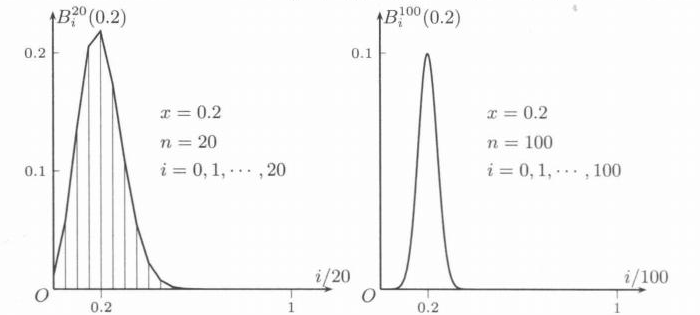
\includegraphics[width=.82\linewidth]{figures/lower/ch16/fig-16-1.png}

  图 16.1
\end{center}

从图上可以看出，将点 $(i/n,B_i^n(0.2))\ (i=0,1,\ldots,n)$ 相连得到的是一条单峰曲线，它的最大值差不多就是 $i/n$ 与 $x=0.2$ 最接近的地方。这一点从概率角度是很直观的事实。我们往往称 $i/n$ 为频率。由于事件 $A$ 出现的概率是 $x=0.2$，平时我们就说成每 5 次独立试验时事件 $A$ 出现 1 次。这当然不可能是完全准确的预言。但是当试验次数 $n$ 越来越大时，频率应当接近 $x=0.2$。这个直观的猜测在概率论中有理论上的证明，这里从略。

对比图 16.1 的两种情况，可以看出当 $n$ 从 $n=20$ 增加到 $n=100$ 时，峰变得越来越窄。这就是说当 $n$ 变大时，频率 $i/n$ 越来越向概率值 $x=0.2$ 靠拢。这种现象在概率论中也有专门讨论。

此外，还要注意恒等式 (16.18) 的概率意义是度量频率偏离概率的程度，在概率论中称为方差。这个恒等式可以用微分法或组合计算得到。其右边的表达式表明当 $n$ 增大时方差是如何降低的。

最后，将和式 (16.16) 分拆的处理表明，在和式中第一个和式是提供接近 $f(x)$ 的主要部分，原因就在于图 16.1 中的单峰现象。而第二个和式则依赖于 (16.18) 来解决。

\begin{xremark}
\textbf{注 1}\quad 虽然 Bernstein 证明有着自己的特点，但从本质上说仍然可以归纳入核函数方法之内。只不过代替卷积的是离散的和式 (16.16)。核函数定义中的三个条件在这里都是满足的。

\textbf{注 2}\quad 关于 Bernstein 多项式在逼近理论中的地位，以及由于 Bézier（贝齐尔）方法的出现而得到新的发展等可以参看数学分析教科书 [8] 的第一册第 5 章。此外，对 Weierstrass 逼近定理的 Bernstein 证明并不一定要从概率角度来理解。Korovkin（科罗夫金）的证明 (1953) 完全从函数论出发，可以参考教科书 [9]。
\end{xremark}

\subsection{逼近定理的一个初等证明}

这里所说的初等证明是指不必使用微积分工具，同时其思路也比较简单。这类证明已有多个。这里介绍的是由 H. Cohen（科恩）给出的证明，见 \textit{Archiv der Mathematik} (1964) 第 15 卷 316--317 页（参见 [53]）。

第一步是对于一个多项式序列的分析。

\begin{xproposition}[16.3.4]
对于任意正数 $\delta\in(0,1/2)$，多项式序列
\[
  Q_n(x)=(1-x^n)^{2n}\qquad(n=1,2,\ldots)
\]
在区间 $[0,\delta]$ 和 $[1-\delta,1]$ 上分别一致收敛于 1 和 0。
\end{xproposition}

\begin{xproof}
在图 16.2 上作出了 $n=1,2,4,10,20$ 的 $Q_n(x)$ 的图像。容易证明
\[
  \lim_{n\to\infty}Q_n\left(\frac12\right)=\frac1\ee\approx0.368.
\]

\begin{center}
  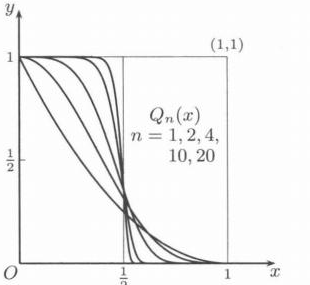
\includegraphics[width=.42\linewidth]{figures/lower/ch16/fig-16-2.png}

  图 16.2
\end{center}

以下的主要工具是 Bernoulli 不等式（见上册第 3 页的命题 1.3.1）：
\[
  \text{当 }h>-1,\ n\in\NN_+\text{ 时，有}\qquad(1+h)^n\geqslant1+nh.
\]
容易看出 $Q_n(x)$ 在区间 $[0,1]$ 上严格单调减少。在区间 $[0,\delta]$ 上
\[
  1\geqslant Q_n(x)\geqslant Q_n(\delta)
  =(1-\delta^n)^{2n}>1-2n\delta^n=1-(2\delta)^n\to1.
\]
又记 $\eta=1-\delta>1/2$，则在区间 $[\eta,1]$ 上，有 $0\leqslant Q_n(x)\leqslant Q_n(\eta)$，且有
\[
  \frac1{Q_n(\eta)}
  =\left(\frac1{1-\eta^n}\right)^{2n}
  =\left(1+\frac{\eta^n}{1-\eta^n}\right)^{2n}
  \geqslant1+\frac{2n\eta^n}{1-\eta^n}>(2\eta)^n\to+\infty.
\]
可见结论成立。
\end{xproof}

作为上述命题的推论就可以得到

\begin{xproposition}[16.3.5]
令 $P_n(x)=Q_n[(1-x)/2],\ n=1,2,\ldots$，则对于任意正数 $\delta\in(0,1)$，多项式序列 $\{P_n\}$ 在 $0<\delta\leqslant|x|\leqslant1$ 上一致收敛于单位跳跃函数（即 Heaviside（赫维塞德）函数）
\[
  H(x)=
  \begin{cases}
    0,&x<0,\\
    1,&x\geqslant0.
  \end{cases}
\]
\end{xproposition}

\paragraph{第一逼近定理的证明}
设 $f\in C[0,1]$，且不妨设 $f(0)=0$。对任意 $\varepsilon>0$，利用关于一致连续性的 Cantor 定理知，存在阶梯函数 $T(x)$，使得在区间 $[0,1]$ 上 $|f(x)-T(x)|<\varepsilon/3$ 成立。利用上述 Heaviside 函数，可以取 $T(x)$ 为
\[
  T(x)=\sum_{k=1}^n s_kH(x-x_k),
\]
其中 $0<x_1<\cdots<x_n<1$，且 $|s_k|<\varepsilon/3,\ k=1,2,\ldots,n$。

现在取 $\delta>0$ 充分小，使得所有区间 $(x_k-\delta,x_k+\delta)\ (k=1,2,\ldots,n)$ 均不相交。然后对于这个 $\delta>0$，根据命题 16.3.5，存在充分大的 $n$，使得成立
\[
  |P_n(x)-H(x)|<\frac{\varepsilon}{3s},\qquad
  \forall\,0<\delta\leqslant|x|\leqslant1,
\]
其中 $s=\sum_{k=1}^n|s_k|$。此外还要注意 $P_n(x)$ 的取值范围必在 0 和 1 之间。

现在构造多项式
\[
  P(x)=\sum_{k=1}^n s_kP_n(x-x_k),
\]
则当 $x$ 属于某个区间 $(x_i-\delta,x_i+\delta)\ (1\leqslant i\leqslant n)$ 时，就有
\[
\begin{aligned}
  |T(x)-P(x)|
  &\leqslant\sum_{k\ne i}|s_k|\,|H(x-x_k)-P_n(x-x_k)|\\
  &\qquad+|s_i|\,|H(x-x_i)-P_n(x-x_i)|\\
  &<s\cdot\frac{\varepsilon}{3s}+|s_i|\cdot1<\frac{2\varepsilon}{3};
\end{aligned}
\]
而当 $x$ 不属于任何 $(x_k-\delta,x_k+\delta)\ (k=1,2,\ldots,n)$ 时，则上述不等式右边只有一项，估计更为简单，即小于 $\varepsilon/3$。

因此就得到
\[
  |f(x)-P(x)|\leqslant|f(x)-T(x)|+|T(x)-P(x)|<\varepsilon.
\]

\subsection{逼近定理的其他证明}

Weierstrass 逼近定理的证法很多，在这里我们将浏览一下其他证明。

首先需要指出两个逼近定理是等价的，即从其中之一可以推出另一个成立。有兴趣的读者可以参考 [1,35,47] 等著作中关于等价性的证明，这里从略。

在第十五章已经用两种方法证明了命题 16.3.2，即第二逼近定理。第一种方法是用 Fejér 核（见命题 15.2.4 的注 2），第二种方法是用 Fourier 级数的一致收敛定理（见命题 15.2.8 的注）。此外，还有在该章参考题 19 中的 de la Vallée Poussin 的证明，它也是一种核方法（参见 [44] 卷 2）。

此外，虽然我们在前面强调了核函数方法的价值，但是从上一小节的证明已经知道，逼近定理有不用核函数方法的初等证明。

对于第一逼近定理，这里较为常见的不用核函数的方法是由 Lebesgue 给出的。其基本思路非常直观。先用分段线性函数来逼近连续函数，然后证明可以将分段线性函数用函数 $f(x)=|x|$ 的平移和 $x$ 的线性组合得到。从而最后问题归结为证明在任意区间 $[a,b]$ 上存在多项式一致逼近 $y=|x|$。这里我们见到的至少有三种方法。第一种方法是利用在例题 14.1.9 介绍的 Visser 定理，它利用迭代方法得到了在 $[-1,1]$ 上一致收敛于 $|x|$ 的多项式序列，而无需微积分工具。第二种方法是在 $(1+x)^{1/2}$ 的 Maclaurin 展开式中将 $x$ 用 $x^2-1$ 代替得到所要的多项式级数展开式。读者可以在 [31,34,47] 找到详细的证明过程。第三种方法是先证明函数列
\begin{equation}
  f_n(x)=\frac{\displaystyle\int_0^x(1-t^2)^n\,\dd t}
  {\displaystyle\int_0^1(1-t^2)^n\,\dd t},\qquad n=1,2,\ldots
\tag{16.20}
\label{eq:16.20}
\end{equation}
对于每个给定的 $\varepsilon\in(0,1)$，在区间 $[-1,-\varepsilon]$ 上和 $[\varepsilon,1]$ 上一致收敛于 $\operatorname{sgn}x$\footnote{这里关于 (16.20) 的结论实际上等价于命题 16.3.5，因此可以按照上一小节的证明做下去。}，然后不难证明函数列
\[
  g_n(x)=\int_0^x f_n(t)\,\dd t,\qquad n=1,2,\ldots
\]
在 $[-1,1]$ 上一致收敛于 $|x|$（参见 [7]）。

最后还应当指出，Weierstrass 逼近定理有许多推广。Weierstrass 本人已经得到高维空间的逼近定理。最有意义的推广是 Stone（斯通）--Weierstrass 定理，它包含了许多逼近定理为其特例，已经成为现代分析的理论支柱之一。读者可以参考在 [14,47] 中的证明，其中后者给出了 Weierstrass 逼近定理的 Stone 证明，它可以几乎不加修改地用于证明 Stone 定理。

\subsection{逼近定理的应用举例}

在举具体例题前需要指出 Weierstrass 逼近定理对于一些基本问题的启示。

首先，在闭区间上的每个连续函数都有用多项式级数或者三角多项式级数的解析表达式，而不需要任何其他条件。因此连续函数与我们过去已经熟悉的可以展开为幂级数的许多初等函数具有共同点：即都可以展开为函数项级数，而且不需要增加其他条件。

有了逼近定理，又可以将连续函数与能够展开为幂级数的函数非常清楚地区分开来。我们已经知道，要将一个函数展开为幂级数，至少要求该函数无限次可导，而且这还不是充分的。一般称这类函数为\textbf{实解析函数}。

如何求出逼近定理中的逼近多项式或三角多项式当然是很重要的问题。这是函数逼近论的研究课题。Weierstrass 逼近定理就是逼近论的最重要的起点。

下面只是逼近定理在数学分析中的几个应用，希望起到抛砖引玉的作用。

\begin{xexample}[16.3.1]
（Lebesgue）证明：区间上的连续函数必有原函数。
\end{xexample}

\begin{xproof}
设 $f\in C[a,b]$，则根据逼近定理知，存在多项式序列 $\{P_n\}$ 于区间 $[a,b]$ 上一致收敛于 $f$。

对每个多项式 $P_n$，存在多项式 $Q_n$，使得在 $[a,b]$ 上满足 $Q_n'=P_n$。同时总可以令 $Q_n(a)=0$ 成立。这样就得到多项式序列 $\{Q_n\}$。

以下分两步，先证明 $\{Q_n\}$ 在 $[a,b]$ 上一致收敛，然后证明其极限函数的导函数就是 $f$。

(1) 根据 $\{P_n\}$ 于 $[a,b]$ 上一致收敛，由 Cauchy 一致收敛准则（的必要性）知道，对于每个 $\varepsilon>0$，存在 $N$，使得对于每个 $n\geqslant N$ 和正整数 $p$，对每个 $x\in[a,b]$ 同时成立
\begin{equation}
  |P_{n+p}(x)-P_n(x)|<\varepsilon.
\tag{16.21}
\label{eq:16.21}
\end{equation}
于是可以在区间 $[a,x]$ 上用 Lagrange 微分中值定理得到
\[
\begin{aligned}
  |Q_{n+p}(x)-Q_n(x)|
  &=|[Q_{n+p}(x)-Q_n(x)]-[Q_{n+p}(a)-Q_n(a)]|\\
  &=|P_{n+p}(\xi)-P_n(\xi)|<\varepsilon.
\end{aligned}
\]
由于这对于所有 $n\geqslant N$ 和正整数 $p$ 以及所有 $x\in[a,b]$ 都成立，再次使用 Cauchy 一致收敛准则（的充分性），就知道 $\{Q_n\}$ 于 $[a,b]$ 一致收敛。记其极限函数为 $F$。它满足条件 $F(a)=0$。

(2) 为了建立 $F'=f$，只需对于每个点 $x_0\in[a,b]$ 和每个给定的 $\varepsilon>0$，证明存在 $\delta>0$，使得当 $0<|h|<\delta$ 时，成立关于差商的不等式
\begin{equation}
  \left|\frac{F(x_0+h)-F(x_0)}h-f(x_0)\right|<3\varepsilon.
\tag{16.22}
\label{eq:16.22}
\end{equation}
这里当然假设 $x_0+h\in[a,b]$。

利用三分法可以将 (16.22) 的左边分拆成
\begin{equation}
\begin{aligned}
  \left|\frac{F(x_0+h)-F(x_0)}h-f(x_0)\right|
  &\leqslant\left|\frac{Q_n(x_0+h)-Q_n(x_0)}h-P_n(x_0)\right|\\
  &\quad+|f(x_0)-P_n(x_0)|\\
  &\quad+\left|\frac{F(x_0+h)-Q_n(x_0+h)-F(x_0)+Q_n(x_0)}h\right|.
\end{aligned}
\tag{16.23}
\label{eq:16.23}
\end{equation}
首先，对于 $\varepsilon>0$，存在 $N$，当 $n\geqslant N$ 时有 $|f(x_0)-P_n(x_0)|<\varepsilon$。又不妨 $N$ 已经足够大，使得对 $n\geqslant N$，对每个正整数 $p$ 和每个 $x\in[a,b]$，不等式 (16.21) 也已经成立。然后在 (16.23) 右边取定 $n=N$。

对固定的 $n=N$，对于 (16.23) 右边的第一项用微分中值定理得到
\[
  \left|\frac{Q_N(x_0+h)-Q_N(x_0)}h-P_N(x_0)\right|
  =|P_N(x_0+\theta h)-P_N(x_0)|,
\]
其中 $0<\theta<1$。利用 $P_N(x)$ 在 $[a,b]$ 上的一致连续性，存在 $\delta>0$，使得当 $|h|<\delta$ 时，上式右边小于 $\varepsilon/3$。

为估计 (16.23) 右边的第三项，先对下列不等式的分子用微分中值定理，得到
\[
\begin{aligned}
&\left|\frac{[Q_{N+p}(x_0+h)-Q_N(x_0+h)]-[Q_{N+p}(x_0)-Q_N(x_0)]}{h}\right|\\
% SOURCE-ERR: 原书此行写作 x+\theta h；按前式及微分中值定理应为 x_0+\theta h。
&\qquad\leqslant|P_{N+p}(x_0+\theta h)-P_N(x_0+\theta h)|<\frac\varepsilon3,
\end{aligned}
\]
其中 $p$ 为任意正整数，$0<\theta<1$，并利用在 $[a,b]$ 一致成立的不等式 (16.21)。最后，在上式左边令 $p\to\infty$，就知道 (16.23) 右边第三项不超过 $\varepsilon$，因此所求证的不等式 (16.22) 成立。
\end{xproof}

\begin{xremark}
这个证明的意义在于，连续函数的原函数的存在性完全不需要定积分概念就可以建立。以上证明是依据 [31] 中的叙述作了改写。（参见按照传统思路安排下的命题 10.3.3。）
\end{xremark}

在 Fourier 级数的收敛性理论中最重要的工具是 Riemann 引理（见例题 10.2.6）。由于在大多数教科书中均有该引理的证明，因此本书在前面对它未作证明。下面是用 Weierstrass 逼近定理的一个证明。

\begin{xexample}[16.3.2]
（Riemann 引理）设 $f\in R[a,b]$，则
\[
  \lim_{p\to+\infty}\int_a^b f(x)\sin px\,\dd x=0,
  \qquad
  \lim_{p\to+\infty}\int_a^b f(x)\cos px\,\dd x=0.
\]
\end{xexample}

\begin{xproof}
只证第一个即可。对于可积函数 $f$ 与每个给定的 $\varepsilon>0$，存在连续函数 $g\in C[a,b]$，使得
\[
  \int_a^b|f(x)-g(x)|\,\dd x<\varepsilon
\]
（见上册第十章第一组参考题 5）。

根据逼近定理，对于 $g$ 存在于 $[a,b]$ 上一致逼近 $g$ 的多项式 $P$，满足
\[
  \int_a^b|g(x)-P(x)|\,\dd x<\varepsilon.
\]
因此就有
\[
  \int_a^b|f(x)-P(x)|\,\dd x
  \leqslant\int_a^b|f(x)-g(x)|\,\dd x
  +\int_a^b|g(x)-P(x)|\,\dd x<2\varepsilon.
\]
然后从
\[
\begin{aligned}
  \left|\int_a^b f(x)\sin px\,\dd x\right|
  &\leqslant\left|\int_a^b[f(x)-P(x)]\sin px\,\dd x\right|
   +\left|\int_a^bP(x)\sin px\,\dd x\right|\\
  &\leqslant\int_a^b|f(x)-P(x)|\,\dd x
   +\left|\int_a^bP(x)\sin px\,\dd x\right|
\end{aligned}
\]
可见，只需要对于多项式证明引理的结论就够了。然而对于连续可微函数的 Riemann 引理的证明特别容易，只需要用分部积分法即可，以下从略。
\end{xproof}

\subsection{练习题}

\begin{xexercise}[1]
设 $f$ 在 $[a,b]$ 上有定义，且对每个 $\varepsilon>0$，存在多项式 $P$，使得满足条件 $|f(x)-P(x)|<\varepsilon,\ \forall x\in[a,b]$，证明：$f\in C[a,b]$。
\end{xexercise}
\begin{xsolution}
任取 $x_0\in[a,b]$ 和 $\varepsilon>0$。由题设可取多项式 $P$，使
\[
  |f(x)-P(x)|<\frac\varepsilon3,
  \qquad x\in[a,b].
\]
多项式 $P$ 在 $x_0$ 连续，所以存在 $\delta>0$，当 $|x-x_0|<\delta$ 且 $x\in[a,b]$ 时，
\[
  |P(x)-P(x_0)|<\frac\varepsilon3.
\]
于是
\[
\begin{aligned}
  |f(x)-f(x_0)|
  &\leqslant|f(x)-P(x)|+|P(x)-P(x_0)|+|P(x_0)-f(x_0)|\\
  &<\varepsilon.
\end{aligned}
\]
故 $f$ 在每个 $x_0\in[a,b]$ 连续，即 $f\in C[a,b]$。
\end{xsolution}


\begin{xexercise}[2]
设 $f\in C[a,b]$，证明：
\begin{enumerate}[label=(\arabic*)]
\item $f$ 可以在 $[a,b]$ 上展开为一致收敛的多项式级数，且在级数中除第一项之外均为在 $[a,b]$ 上非负的多项式；
\item $f$ 可以在 $[a,b]$ 上展开为绝对一致收敛的多项式级数；
\item 对于给定的收敛正项级数 $\sum_{n=1}^{\infty}a_n$，其中有无限多项大于 0，存在于区间 $[a,b]$ 上一致收敛于 $f$ 的多项式级数 $\sum_{n=1}^{\infty}P_n(x)$，使满足条件
\[
  \sup_{x\in[a,b]}\{|P_n(x)|\}\leqslant a_n,
  \qquad \forall n=1,2,\ldots.
\]
\end{enumerate}
\end{xexercise}
\begin{xsolution}
\textbf{(1)}\quad
由 Weierstrass 逼近定理，可取多项式 $R_n$，使
\[
  \|f-R_n\|_\infty\leqslant4^{-n},\qquad n=1,2,\ldots.
\]
对 $n\geqslant2$ 令
\[
  D_n=R_n-R_{n-1},\qquad
  c_n=\max\left\{0,-\min_{x\in[a,b]}D_n(x)\right\}.
\]
则 $D_n+c_n\geqslant0$ 于 $[a,b]$ 上恒成立，且
\[
  0\leqslant c_n\leqslant\|D_n\|_\infty
  \leqslant4^{-n}+4^{-(n-1)}.
\]
因此 $C=\sum_{n=2}^{\infty}c_n<\infty$。定义
\[
  P_1=R_1-C,
  \qquad P_n=D_n+c_n\quad(n\geqslant2).
\]
则 $P_n$（$n\geqslant2$）都是在 $[a,b]$ 上非负的多项式，并且
\[
  \sum_{n=1}^NP_n
  =R_N-\sum_{n=N+1}^{\infty}c_n.
\]
右边一致收敛于 $f$，故
\[
  f=\sum_{n=1}^{\infty}P_n
\]
在 $[a,b]$ 上一致收敛，且除第一项外各项均非负。

\textbf{(2)}\quad
仍取多项式 $R_n$ 使 $\|f-R_n\|_\infty\leqslant4^{-n}$。令
\[
  P_1=R_1,
  \qquad P_n=R_n-R_{n-1}\quad(n\geqslant2).
\]
则 $\sum_{k=1}^NP_k=R_N\to f$ 一致。并且
\[
\begin{aligned}
  \sum_{n=1}^{\infty}\|P_n\|_\infty
  &\leqslant\|R_1\|_\infty
  +\sum_{n=2}^{\infty}
  \bigl(\|R_n-f\|_\infty+\|R_{n-1}-f\|_\infty\bigr)\\
  &<+\infty.
\end{aligned}
\]
故该多项式级数绝对一致收敛于 $f$。

\textbf{(3)}\quad
按原书现有题面，此命题不能成立。事实上若
\[
  f(x)\equiv M,\qquad
  M>\sum_{n=1}^{\infty}a_n,
\]
而又存在题设级数，则由一致收敛及三角不等式必有
\[
  M=|f(x)|
  =\left|\sum_{n=1}^{\infty}P_n(x)\right|
  \leqslant\sum_{n=1}^{\infty}\sup_{t\in[a,b]}|P_n(t)|
  \leqslant\sum_{n=1}^{\infty}a_n,
\]
矛盾。因此原题至少缺少一个必要条件，不能在不改动题意的情况下给出所要求的证明。
\end{xsolution}


\begin{xexercise}[3]
设 $f\in R[a,b]$，则对于每个 $\varepsilon>0$，存在两个多项式 $p(x)$ 和 $P(x)$，使得满足条件：
\begin{enumerate}[label=(\arabic*)]
\item $p(x)\leqslant f(x)\leqslant P(x),\ \forall x\in[a,b]$；
\item $\displaystyle\int_a^b[P(x)-p(x)]\,\dd x<\varepsilon$。
\end{enumerate}
\end{xexercise}
\begin{xsolution}
设 $f\in R[a,b]$。任取 $\varepsilon>0$。由 Riemann 可积性，可取分割
\[
  a=x_0<x_1<\cdots<x_m=b,
\]
使上、下 Darboux 和之差小于 $\varepsilon/3$。在每个小区间记
\[
  M_i=\sup_{[x_{i-1},x_i]}f,
  \qquad m_i=\inf_{[x_{i-1},x_i]}f.
\]
于是阶梯函数 $u,l$ 满足 $l\leqslant f\leqslant u$ 且
\[
  \int_a^b(u-l)\,\dd x<\frac\varepsilon3.
\]

设 $M=\sup_{[a,b]}f$，$m=\inf_{[a,b]}f$。在各分点的充分小邻域内，把 $u$ 向上用常值 $M$ 连接，把 $l$ 向下用常值 $m$ 连接，并在邻域边缘作线性连接；邻域总长度可任意小。因此可构造连续函数 $U,L$，满足
\[
  L\leqslant l\leqslant f\leqslant u\leqslant U,
  \qquad
  \int_a^b(U-L)\,\dd x<\frac{2\varepsilon}{3}.
\]
（这里多出的积分只发生在有限个分点的这些小邻域中，所以可通过缩小邻域使之任意小。）

由 Weierstrass 逼近定理，取多项式 $P_0,p_0$，使
\[
  \|P_0-U\|_\infty<\delta,
  \qquad \|p_0-L\|_\infty<\delta,
\]
其中选 $2\delta(b-a)<\varepsilon/3$。令
\[
  P=P_0+\delta,\qquad p=p_0-\delta.
\]
则
\[
  p\leqslant L\leqslant f\leqslant U\leqslant P
\]
在 $[a,b]$ 上处处成立，且
\[
\begin{aligned}
  \int_a^b[P(x)-p(x)]\,\dd x
  &\leqslant\int_a^b[U(x)-L(x)]\,\dd x+2\delta(b-a)\\
  &<\varepsilon.
\end{aligned}
\]
两项要求均得证。
\end{xsolution}


\begin{xexercise}[4]
设 $f\in C[a,b]$，且对每个非负整数 $n$ 满足条件 $\int_a^b x^nf(x)\,\dd x=0$，证明：$f$ 为恒等于 0 的常值函数。又若条件改为对于大于某个正整数 $n_0$ 的所有 $n$ 成立，则也有相同结论。
\end{xexercise}
\begin{xsolution}
先设对所有 $n\geqslant0$ 都有
\[
  \int_a^bx^nf(x)\,\dd x=0.
\]
于是对任意多项式 $P$ 都有 $\int_a^bP(x)f(x)\,\dd x=0$。由 Weierstrass 定理取多项式 $P_k\to f$ 一致，则
\[
  \int_a^bf(x)^2\,\dd x
  =\lim_{k\to\infty}\int_a^bf(x)P_k(x)\,\dd x=0.
\]
$f^2$ 连续且非负，故 $f\equiv0$。

若只知道对所有 $n>n_0$ 成立，令
\[
  g(x)=x^{n_0+1}f(x).
\]
则对每个 $k\geqslant0$，
\[
  \int_a^bx^kg(x)\,\dd x
  =\int_a^bx^{k+n_0+1}f(x)\,\dd x=0.
\]
由上一步 $g\equiv0$。因此当 $x\ne0$ 时 $f(x)=0$；若 $0\in[a,b]$，再由连续性得 $f(0)=0$。故仍有 $f\equiv0$。
\end{xsolution}


\begin{xexercise}[5]
\begin{enumerate}[label=(\arabic*)]
\item 设 $f\in C[-1,1]$，且对每个非负整数 $n$ 满足条件 $\int_{-1}^1x^{2n}f(x)\,\dd x=0$，则 $f$ 必为奇函数；
\item 设 $f\in C[-1,1]$，且对每个非负整数 $n$ 满足条件 $\int_{-1}^1x^{2n+1}f(x)\,\dd x=0$，则 $f$ 必为偶函数。
\end{enumerate}
\end{xexercise}
\begin{xsolution}
\textbf{(1)}\quad
写成偶、奇部分
\[
  f=f_e+f_o,
  \qquad
  f_e(x)=\frac{f(x)+f(-x)}2.
\]
因为 $x^{2n}f_o(x)$ 为奇函数，题设等价于
\[
  \int_{-1}^1x^{2n}f_e(x)\,\dd x=0,
  \qquad n=0,1,\ldots.
\]
$f_e$ 为偶连续函数。令 $h(t)=f_e(\sqrt t)$（$0\leqslant t\leqslant1$），则 $h$ 连续。由 Weierstrass 定理可取多项式 $Q_k(t)$ 一致逼近 $h(t)$，于是 $Q_k(x^2)$ 一致逼近 $f_e(x)$，且每个 $Q_k(x^2)$ 都是偶次幂的线性组合。因此
\[
  \int_{-1}^1f_e(x)Q_k(x^2)\,\dd x=0.
\]
令 $k\to\infty$ 得
\[
  \int_{-1}^1f_e(x)^2\,\dd x=0,
\]
所以 $f_e\equiv0$。于是 $f=f_o$ 为奇函数。

\textbf{(2)}\quad
仍写 $f=f_e+f_o$。因 $x^{2n+1}f_e(x)$ 为奇函数，题设给出
\[
  \int_{-1}^1x^{2n+1}f_o(x)\,\dd x=0,
  \qquad n=0,1,\ldots.
\]
令 $g(x)=xf_o(x)$。则 $g$ 是偶连续函数，且
\[
  \int_{-1}^1x^{2n}g(x)\,\dd x=0,
  \qquad n=0,1,\ldots.
\]
按题 5(1) 的偶函数论证可得 $g\equiv0$，故 $f_o(x)=0$ 对 $x\ne0$ 成立，而 $f_o(0)=0$。因此 $f_o\equiv0$，即 $f$ 为偶函数。
\end{xsolution}


\begin{xexercise}[6]
设 $f\in C[0,1]$，证明：存在每项为奇次项的多项式序列在 $[0,1]$ 上一致收敛于 $f$ 的充分必要条件为 $f(0)=0$。
\end{xexercise}
\begin{xsolution}
必要性立即成立：每个只含奇次项的多项式在 $x=0$ 处都等于 0，一致极限也必须满足 $f(0)=0$。

反之，设 $f(0)=0$。在 $[-1,1]$ 上作奇延拓
\[
  F(x)=
  \begin{cases}
    f(x),&0\leqslant x\leqslant1,\\
    -f(-x),&-1\leqslant x<0.
  \end{cases}
\]
由 $f(0)=0$，$F\in C[-1,1]$ 且 $F$ 为奇函数。由 Weierstrass 定理，对任意 $n$ 可取多项式 $P_n$ 使 $P_n\to F$ 一致。令
\[
  Q_n(x)=\frac{P_n(x)-P_n(-x)}2.
\]
则 $Q_n$ 是只含奇次项的多项式，并且
\[
  |Q_n(x)-F(x)|
  \leqslant\frac{|P_n(x)-F(x)|+|P_n(-x)-F(-x)|}{2}
  \to0
\]
一致成立。限制到 $[0,1]$ 即得所需序列。
\end{xsolution}


\begin{xexercise}[7]
设 $f\in R[a,b]$，且对每个非负整数 $n$ 满足条件 $\int_a^b x^nf(x)\,\dd x=0$，证明：$f$ 在每个连续点上等于 0。
\end{xexercise}
\begin{xsolution}
由题设，对每个多项式 $P$ 都有
\[
  \int_a^bf(x)P(x)\,\dd x=0.
\]
任取 $g\in C[a,b]$。由 Weierstrass 定理取多项式 $P_k\to g$ 一致。因 $f$ Riemann 可积故有界，于是
\[
  \int_a^bf(x)g(x)\,\dd x
  =\lim_{k\to\infty}\int_a^bf(x)P_k(x)\,\dd x=0.
\]

若 $x_0$ 是 $f$ 的连续点而 $f(x_0)>0$，则存在小闭区间 $I\ni x_0$ 和常数 $c>0$，使 $f(x)\geqslant c$ 于 $I$ 上。取非负连续函数 $g$，其支集包含于 $I$ 且不恒为 0，则
\[
  \int_a^bf(x)g(x)\,\dd x\geqslant c\int_Ig(x)\,\dd x>0,
\]
与上式矛盾。$f(x_0)<0$ 同理。故每个连续点 $x_0$ 都有 $f(x_0)=0$。
\end{xsolution}


\begin{xexercise}[8]
设函数 $f$ 在区间 $(-\infty,+\infty)$ 上可以展开为一致收敛的多项式级数，证明：$f$ 本身必是多项式。（这断定了 Weierstrass 定理不可能不作改变而推广到无限区间上去。）
\end{xexercise}
\begin{xsolution}
设
\[
  f(x)=\sum_{n=1}^{\infty}P_n(x)
\]
在整个 $\RR$ 上一致收敛，部分和记为 $S_N$。由一致 Cauchy 准则，存在 $N_0$，使得对任意 $m,n\geqslant N_0$，
\[
  \sup_{x\in\RR}|S_m(x)-S_n(x)|<1.
\]
但 $S_m-S_n$ 是多项式；一个非恒定多项式在 $\RR$ 上必无界，因此 $S_m-S_n$ 只能是常数。固定 $n=N_0$，可写
\[
  S_m(x)=S_{N_0}(x)+c_m,
  \qquad m\geqslant N_0.
\]
由一致收敛（在任一点取值即可）知 $c_m\to c$，于是
\[
  f(x)=S_{N_0}(x)+c,
\]
本身是多项式。
\end{xsolution}


\section{用级数构造函数}

无穷级数不仅是研究函数的工具，而且可以用于构造出具有各种特殊性质的函数，其中有不少例子在数学发展史上起了重要的作用。

这里应当指出，认为这些“病态”函数只是用作反例而没有其他意义的观点早已过时。与 §5.6 介绍的混沌几乎同时发展起来的另一个新的非线性科学领域是“分形”(fractal)，其中的主要角色就是包括本节内容在内的各种“怪物”。对此有兴趣的读者可以参考 [32,20]。

\subsection{处处连续处处不可微的函数}

在很长时间内人们对于连续性与可微性之间的关系不清楚，许多人猜测连续函数只会在个别点或很少的点上不可微。由于举出了处处连续处处不可微函数的例子，这个问题得到了彻底解决。

这类例子最早出现在 Bolzano 的 1830 年的手稿中，但只有曲线，并无解析表达式，也没有证明（见 [15]）。正式发表并有严格证明的第一个例子则属于 Weierstrass (1872 年)（可参考 [15,26,29] 等）。

\textbf{Weierstrass 函数}是一个缺项 Fourier 级数：
\[
  F(x)=\sum_{n=1}^{\infty}a^n\sin(b^n\pi x),
\]
其中 $b$ 为奇数，$0<a<1$，且 $ab>1+3\pi/2$。由于右边的级数一致收敛，因此函数 $F$ 的连续性是明显的。关于 $F$ 处处不可微的证明可以在 [51,29] 中找到。

目前教科书中在介绍处处连续处处不可微函数时一般均用 van der Waerden（范德瓦尔登）于 1930 年提出的例子。它在几何上相当直观，证明也比较简单。下面的证明可能比 [18] 第二卷的 444 小节更简单一些。主要工具是利用关于差商的一个简单命题\footnote{证明是简单的，用上册 159 页的无穷小增量公式 (6.1) 即可。当然这里要求对每个 $n$ 成立 $b_n-a_n>0$。又参见上册 189 页。}：若函数 $f$ 于点 $x_0$ 可导，且 $\{[a_n,b_n]\}$ 是以点 $x_0$ 为惟一公共点的闭区间套，则就有
\begin{equation}
  \lim_{n\to\infty}\frac{f(b_n)-f(a_n)}{b_n-a_n}=f'(x_0).
\tag{16.24}
\label{eq:16.24}
\end{equation}

与 Weierstrass 函数类似，van der Waerden 函数是用无穷级数来构造的。现在按照下列步骤定义这个无穷级数的通项 $\{f_n\}$：
\begin{enumerate}[label=\arabic*.]
\item 将区间 $[-1,1]$ 上的函数 $f(x)=|x|$ 按周期 2 延拓成为 $(-\infty,+\infty)$ 上的周期连续函数，仍记为 $f$。
\item 以 $f$ 为模板构造函数列 $\{f_n\}$：
\begin{equation}
  f_n(x)=\frac1{2^n}f(2^nx),\qquad n=1,2,\ldots,\quad x\in(-\infty,+\infty).
\tag{16.25}
\label{eq:16.25}
\end{equation}
可以看出 $f_n$ 为周期 $1/2^{n-1}$ 的连续周期函数，且有 $0\leqslant f_n(x)\leqslant1/2^n$。还可以看出 $f_n$ 的极值点等距分布，相邻极值点之间的距离也是 $1/2^n$。
\item 重要的是 $f_n$ 与 $f_{n+1}$ 之间有如下的关系：
\begin{enumerate}[label=(\arabic*)]
\item $f_n$ 的极值点必是 $f_{n+1}$ 的零点；
\item $f_{n+1}$ 的任意两个相邻极值点必落在 $f_n$ 为线性的一个子区间内。
\end{enumerate}
\item 对任意正整数 $n$，设 $a_n,b_n$ 为 $f_n$ 的任意两个相邻的极值点，则
\begin{enumerate}[label=(\arabic*)]
\item $k>n$ 时，由 3.(1) 知 $a_n,b_n$ 为 $f_k$ 的零点，因此
\begin{equation}
  \frac{f_k(a_n)-f_k(b_n)}{a_n-b_n}=0.
\tag{16.26}
\label{eq:16.26}
\end{equation}
\item $k\leqslant n$ 时，由 3.(2) 知
\begin{equation}
  \frac{f_k(a_n)-f_k(b_n)}{a_n-b_n}=1\quad\text{或}\quad-1.
\tag{16.27}
\label{eq:16.27}
\end{equation}
\end{enumerate}
\end{enumerate}

以上关于 $\{f_n\}$ 的性质非常直观，读者可以对照图 16.3(a) 中对于 $f_1,f_2,f_3$ 在区间 $[0,1]$ 上的曲线段来理解这些性质。

现在定义 van der Waerden 函数如下：
\begin{equation}
  W(x)=\sum_{n=1}^{\infty}f_n(x),\qquad x\in(-\infty,+\infty).
\tag{16.28}
\label{eq:16.28}
\end{equation}
从 $|f_n(x)|\leqslant1/2^n$ 可知 (16.28) 右边的函数项级数一致收敛，因此和函数 $W(x)$ 在 $(-\infty,+\infty)$ 内处处连续。最后，我们来证明：

\begin{xproposition}[16.4.1]
连续函数 $W$ 在 $(-\infty,+\infty)$ 内处处不可导。
\end{xproposition}

\begin{xproof}
对任意指定的点 $x_0$，由 (16.24) 可知，只要能找到以 $x_0$ 为惟一公共点的闭区间套 $\{[a_n,b_n]\}$，使得极限
\[
  \lim_{n\to\infty}\frac{W(b_n)-W(a_n)}{b_n-a_n}
\]
不存在即可。

利用 $f_n$ 的极值点等距分布，且相邻极值点的距离为 $1/2^n$，取 $a_n$ 和 $b_n$ 为 $f_n$ 的两个极值点，满足条件：(1) $a_n\leqslant x_0\leqslant b_n$；(2) $b_n-a_n=1/2^n$。

记
\[
  d_n=\frac{W(b_n)-W(a_n)}{b_n-a_n},\qquad n=1,2,\ldots,
\]
则
\[
\begin{aligned}
  d_n
  &=\frac1{b_n-a_n}\left(\sum_{k=1}^{\infty}f_k(b_n)-\sum_{k=1}^{\infty}f_k(a_n)\right)\\
  &=\sum_{k=1}^{\infty}\frac{f_k(b_n)-f_k(a_n)}{b_n-a_n}.
\end{aligned}
\]
由式 (16.26) 知上式右边和式中的项当 $k>n$ 时均为 0，因此有
\[
  d_n=\sum_{k=1}^n\frac{f_k(b_n)-f_k(a_n)}{b_n-a_n}.
\]
由式 (16.27) 知上式右边和式的每一项为 $-1$ 或 1。因此当 $n$ 为偶数时 $d_n$ 为偶整数，而当 $n$ 为奇数时 $d_n$ 为奇整数。由此可见这样的数列 $\{d_n\}$ 一定发散，从而函数 $W$ 在点 $x_0$ 处不可导。
\end{xproof}

\begin{center}
  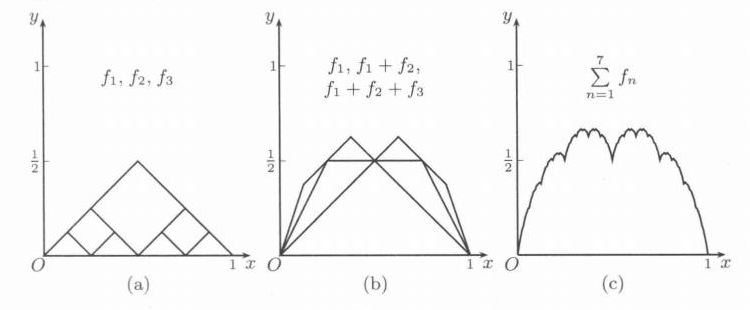
\includegraphics[width=.88\linewidth]{figures/lower/ch16/fig-16-3.png}

  图 16.3
\end{center}

\begin{xremark}
\textbf{注 1}\quad 在图 16.3(b),(c) 中分别作出了 (16.28) 右边级数的前 3 个和第 7 个部分和函数，后者与 $W(x)$ 已很接近。读者可以结合证明来理解 van der Waerden 函数处处不可导的直观原因。在 [18] 等著作中一般是证明两个单侧导数都不存在，讨论比这里要更细致一点。此外，在定义 $f_n$ 的公式 (16.25) 中的比例因子 $2^n$ 改为 $4^n$ 或 $10^n$ 都是可以的。在 [15] 中的证明则完全不依赖于几何直观，也可供参考。

\textbf{注 2}\quad 这方面的工作很多，较近的成果见《美国数学月刊》(2002) 第 109 卷 378--380 页上的一文及其中的文献。
\end{xremark}

\subsection{填满正方形的连续曲线}

Cantor 首先证明：直线上的所有点全体和平面上的所有点全体之间存在一一对应，同样在区间 $[0,1]$ 内的所有点全体和单位正方形 $[0,1;0,1]$ 内的所有点全体之间也存在一一对应。

填满正方形的连续曲线就是将区间 $[0,1]$ 连续映射到单位正方形的满射。Peano 在 1890 年第一次构造出了这样的例子。此后人们经常将这类曲线称为 Peano 曲线。它使我们对于如何合理定义曲线的概念起了重要的推动作用（参见 [5,31]）。这里要注意，Peano 曲线一定有自交点。这是因为在 $[0,1]$ 和 $[0,1;0,1]$ 之间的一一映射不可能是连续的。

下面这个例子是 1938 年由 Schoenberg（舍恩贝格）作出的。显然，这样的曲线需要用参数方程
\[
  x=x(t),\qquad y=y(t),\qquad t\in[0,1]
\]
来表示。定义
\[
  \varphi(t)=
  \begin{cases}
    0,&t\in[0,1/3],\\
    3t-1,&t\in(1/3,2/3],\\
    1,&t\in(2/3,1].
  \end{cases}
\]
按照
\[
  \varphi(t)=\varphi(-t),\qquad \varphi(t+2)=\varphi(t),\qquad t\in(-\infty,+\infty)
\]
将 $\varphi(t)$ 延拓到 $(-\infty,+\infty)$ 上，再令
\[
  x(t)=\sum_{n=1}^{\infty}\frac{\varphi(3^{2n-2}t)}{2^n},\qquad
  y(t)=\sum_{n=1}^{\infty}\frac{\varphi(3^{2n-1}t)}{2^n},\qquad t\in[0,1].
\]
这就是所要作的曲线。将正方形 $[0,1;0,1]$ 中每个点的坐标 $(x,y)$ 用二进制展开就不难证明存在 $t\in[0,1]$，使得 $x(t)=x,y(t)=y$（可以参看 [8,15] 等）。

\section{对于教学的建议}

\subsection{学习要点}

本章只是对于前三章的补充，在教学中可根据情况选用。

\begin{enumerate}[label=\arabic*.]
\item 在许多积分计算中无穷级数经常有用，它在求出有限形式答案和近似计算方面都是不可缺少的手段。这里的问题已经与含参数量的积分有关，但其中的参数只是离散的正整数。
\item 级数求和有很多内容，§16.2 列出的都是常用方法。关于幂级数求和的材料见 14.3.3 小节的例题，这里不再叙述。
\item Weierstrass 逼近定理在教科书中都有，但一般只举出一种证法。§16.3 对此给出一个综述，同时还对其应用举例。
\item 利用无穷级数构造具有特殊性质的函数是个经典问题。这方面可用下面的几个参考题进行训练。
\end{enumerate}

\subsection{参考题}

\begin{xreferenceproblem}[1]
求下列级数之和：
\begin{enumerate}[label=(\arabic*)]
\item $\displaystyle\frac1{1\cdot2\cdot3}+\frac1{3\cdot4\cdot5}+\frac1{5\cdot6\cdot7}+\cdots$；
\item $\displaystyle\frac1{2\cdot3\cdot4}+\frac1{4\cdot5\cdot6}+\frac1{6\cdot7\cdot8}+\cdots$；
\item $\displaystyle\frac1{1\cdot2\cdot3\cdot4}+\frac1{4\cdot5\cdot6\cdot7}+\frac1{7\cdot8\cdot9\cdot10}+\cdots$。
\end{enumerate}
\end{xreferenceproblem}
\begin{xsolution}
\textbf{(1)}\quad
用 Beta 积分
\[
  \frac1{m(m+1)(m+2)}
  =\frac12\int_0^1x^{m-1}(1-x)^2\,\dd x.
\]
取 $m=2k+1$ 并求和：
\[
\begin{aligned}
S&=\frac12\int_0^1(1-x)^2\sum_{k=0}^{\infty}x^{2k}\,\dd x\\
 &=\frac12\int_0^1\frac{1-x}{1+x}\,\dd x
 =\ln2-\frac12.
\end{aligned}
\]

\textbf{(2)}\quad
同样取 $m=2k+2$：
\[
\begin{aligned}
S&=\frac12\int_0^1(1-x)^2\sum_{k=0}^{\infty}x^{2k+1}\,\dd x\\
 &=\frac12\int_0^1\frac{x(1-x)}{1+x}\,\dd x\\
 &=\frac34-\ln2.
\end{aligned}
\]

\textbf{(3)}\quad
有
\[
  \frac1{m(m+1)(m+2)(m+3)}
  =\frac16\int_0^1x^{m-1}(1-x)^3\,\dd x.
\]
令 $m=3k+1$，则
\[
\begin{aligned}
S&=\frac16\int_0^1\frac{(1-x)^3}{1-x^3}\,\dd x
 =\frac16\int_0^1\frac{(1-x)^2}{1+x+x^2}\,\dd x\\
 &=\frac16\left(1-\frac32\ln3+\frac{\pi}{2\sqrt3}\right).
\end{aligned}
\]
即
\[
  S=\frac16-\frac14\ln3+\frac{\pi}{12\sqrt3}.
\]
\end{xsolution}


\begin{xreferenceproblem}[2]
求 Leibniz 型级数 $\displaystyle\sum_{n=1}^{\infty}(-1)^{n-1}\frac{\ln n}{n}$ 之和。
\end{xreferenceproblem}
\begin{xsolution}
记
\[
  S_N=\sum_{k=1}^{N}(-1)^{k-1}\frac{\ln k}{k}.
\]
由于 $\ln k/k$ 从充分大的 $k$ 起单调趋于 $0$，原级数由 Leibniz 判别法收敛。考察偶数部分和：
\[
\begin{aligned}
  S_{2n}
  &=\sum_{k=1}^{2n}\frac{\ln k}{k}
    -2\sum_{k=1}^{n}\frac{\ln(2k)}{2k}\\
  &=\sum_{k=n+1}^{2n}\frac{\ln k}{k}
    -\ln2\sum_{k=1}^{n}\frac1k.
\end{aligned}
\]
把第一项写成 Riemann 和：
\[
\begin{aligned}
  \sum_{k=n+1}^{2n}\frac{\ln k}{k}
  &=\frac1n\sum_{j=1}^{n}
    \frac{\ln(1+j/n)}{1+j/n}
    +\ln n\sum_{j=1}^{n}\frac1{n+j}.
\end{aligned}
\]
于是
\[
\begin{aligned}
  S_{2n}
  &=\frac1n\sum_{j=1}^{n}
    \frac{\ln(1+j/n)}{1+j/n}\\
  &\quad+\ln n\left(H_{2n}-H_n-\ln2\right)
    +\ln2\left(\ln n-H_n\right),
\end{aligned}
\]
其中 $H_n=\sum_{k=1}^n1/k$。第一项趋于
\[
  \int_0^1\frac{\ln(1+x)}{1+x}\,\dd x
  =\frac{(\ln2)^2}{2}.
\]
又由 $H_n-\ln n\to\gamma$，以及
\[
  H_{2n}-H_n-\ln2=\bigO\left(\frac1n\right),
\]
可知第二项趋于 $0$，第三项趋于 $-\gamma\ln2$。因此
\[
  \boxed{\displaystyle
  \sum_{n=1}^{\infty}(-1)^{n-1}\frac{\ln n}{n}
  =\frac{(\ln2)^2}{2}-\gamma\ln2 }.
\]
\end{xsolution}


\begin{xreferenceproblem}[3]
证明：
\[
  \sum_{m=1}^{\infty}\sum_{\substack{n=1\\n\ne m}}^{\infty}\frac1{m^2-n^2}=-\frac{\pi^2}{8}.
\]
\end{xreferenceproblem}
\begin{xsolution}
固定 $m\geqslant1$，先算内层级数。对 $N>m$，
\[
\begin{aligned}
\sum_{\substack{n=1\\n\ne m}}^N\frac1{m^2-n^2}
&=\frac1{2m}\sum_{\substack{n=1\\n\ne m}}^N
 \left(\frac1{m-n}+\frac1{m+n}\right)\\
&=\frac1{2m}\left(
H_{m-1}-H_{N-m}+H_{N+m}-H_m-\frac1{2m}
\right).
\end{aligned}
\]
令 $N\to\infty$，因 $H_{N+m}-H_{N-m}\to0$，得
\[
  \sum_{\substack{n=1\\n\ne m}}^{\infty}\frac1{m^2-n^2}
  =-\frac3{4m^2}.
\]
因此
\[
\begin{aligned}
  \sum_{m=1}^{\infty}\sum_{\substack{n=1\\n\ne m}}^{\infty}
  \frac1{m^2-n^2}
  &=-\frac34\sum_{m=1}^{\infty}\frac1{m^2}
  =-\frac{\pi^2}{8}.
\end{aligned}
\]
\end{xsolution}


\begin{xreferenceproblem}[4]
（Goldbach 哥德巴赫）设 $q$ 取遍所有大于 1 的正整数的乘幂，且其指数均大于 1，证明：
\[
  \sum_q\frac1{q-1}=1.
\]
\end{xreferenceproblem}
\begin{xsolution}
设 $\mathcal P$ 为所有不同的完全幂 $q=a^r$（$a>1,r>1$）的集合。由于各项非负，可自由交换求和：
\[
  \sum_{q\in\mathcal P}\frac1{q-1}
  =\sum_{q\in\mathcal P}\sum_{j=1}^{\infty}\frac1{q^j}.
\]
另一方面，
\[
  \sum_{a=2}^{\infty}\frac1{a(a-1)}
  =\sum_{a=2}^{\infty}\sum_{r=2}^{\infty}\frac1{a^r}=1.
\]
下面说明这两个双重正项级数逐整数计数完全相同。

任一整数 $N>1$ 可唯一写成
\[
  N=c^d,
\]
其中 $c$ 不是完全幂，$d$ 是 $N$ 的素因子指数的最大公约数。若 $d=1$，$N$ 在两边都不出现。若 $d\geqslant2$，则右边 $\sum_{a,r}$ 中 $1/N$ 出现的次数等于 $d$ 的大于 1 的正因子个数（每个 $r\mid d,r>1$ 给出 $a=c^{d/r}$）。左边 $\sum_{q,j}$ 中 $1/N$ 出现的次数也等于这个数：$q=c^e$ 必有 $e\mid d,e>1$，而 $j=d/e$。因此两边每个 $1/N$ 的重数相同。

故
\[
  \sum_{q\in\mathcal P}\frac1{q-1}
  =\sum_{a=2}^{\infty}\frac1{a(a-1)}=1.
\]
\end{xsolution}


\begin{xreferenceproblem}[5]
设 $a_1=2,a_2=8,a_n=4a_{n-1}-a_{n-2},\ n=3,4,5,\ldots$，证明：
\[
  \sum_{n=1}^{\infty}\operatorname{arccot}a_n^2=\frac\pi{12}.
\]
\end{xreferenceproblem}
\begin{xsolution}
把递推式向前延拓令 $a_0=0$，则
\[
  a_{n+1}+a_{n-1}=4a_n.
\]
还可由递推式归纳得到
\[
  a_n^2-a_{n-1}a_{n+1}=4.
\]
令
\[
  \theta_n=\arctan\frac{a_n}{a_{n+1}},\qquad \theta_0=0.
\]
则
\[
\begin{aligned}
  \tan(\theta_n-\theta_{n-1})
  &=\frac{a_n^2-a_{n-1}a_{n+1}}
  {a_n(a_{n+1}+a_{n-1})}\\
  &=\frac4{4a_n^2}=\frac1{a_n^2}.
\end{aligned}
\]
而 $0<\theta_n-\theta_{n-1}<\pi/2$，故
\[
  \operatorname{arccot}a_n^2
  =\arctan\frac1{a_n^2}=\theta_n-\theta_{n-1}.
\]
递推方程特征根为 $2\pm\sqrt3$，所以
\[
  \frac{a_n}{a_{n+1}}\to2-\sqrt3=\tan\frac\pi{12}.
\]
望远镜求和即得
\[
  \sum_{n=1}^{\infty}\operatorname{arccot}a_n^2
  =\lim_{N\to\infty}\theta_N=\frac\pi{12}.
\]
\end{xsolution}


\begin{xreferenceproblem}[6]
证明：
\[
  \pi=\sum_{n=0}^{\infty}\frac{(n!)^2 2^{2n+1}}{(2n+1)!}.
\]
\end{xreferenceproblem}
\begin{xsolution}
按原书扫描题面，应证明
\[
  \pi=\sum_{n=0}^{\infty}
  \frac{(n!)^2 2^{n+1}}{(2n+1)!}.
\]
由 Beta 积分
\[
  \frac{(n!)^2}{(2n+1)!}
  =\int_0^1x^n(1-x)^n\,\dd x.
\]
各项非负，所以
\[
\begin{aligned}
  \sum_{n=0}^{\infty}\frac{(n!)^22^{n+1}}{(2n+1)!}
  &=2\int_0^1\sum_{n=0}^{\infty}[2x(1-x)]^n\,\dd x\\
  &=2\int_0^1\frac{\dd x}{1-2x(1-x)}.
\end{aligned}
\]
令 $u=2x-1$，则
\[
  1-2x(1-x)=\frac{1+u^2}{2},\qquad \dd x=\frac12\dd u,
\]
于是
\[
  2\int_0^1\frac{\dd x}{1-2x(1-x)}
  =2\int_{-1}^1\frac{\dd u}{1+u^2}=\pi.
\]
\end{xsolution}


\begin{xreferenceproblem}[7]
设 $\{g_n\}$ 是 $[0,1]$ 上非负连续函数列，且对每个 $x^k\ (k=0,1,\ldots)$ 存在极限
\[
  \lim_{n\to\infty}\int_0^1x^kg_n(x)\,\dd x,
\]
证明：对任意的 $f\in C[0,1]$，存在极限
\[
  \lim_{n\to\infty}\int_0^1f(x)g_n(x)\,\dd x.
\]
\end{xreferenceproblem}
\begin{xsolution}
由 $k=0$ 的假设，数列
\[
  \int_0^1g_n(x)\,\dd x
\]
有极限，因此存在常数 $M>0$，使
\[
  \int_0^1g_n(x)\,\dd x\leqslant M
\]
对所有 $n$ 成立。

任取 $f\in C[0,1]$ 和 $\varepsilon>0$。由 Weierstrass 定理取多项式
\[
  P(x)=\sum_{k=0}^ma_kx^k
\]
使 $\|f-P\|_\infty<\varepsilon/(3M)$。则
\[
  \left|\int_0^1(f-P)g_n\,\dd x\right|
  \leqslant\|f-P\|_\infty\int_0^1g_n\,\dd x<\frac\varepsilon3.
\]
而
\[
  \int_0^1P(x)g_n(x)\,\dd x
  =\sum_{k=0}^ma_k\int_0^1x^kg_n(x)\,\dd x
\]
按假设有极限，故为 Cauchy 数列。于是充分大的 $m,n$ 有
\[
  \left|\int_0^1P(g_m-g_n)\,\dd x\right|<\frac\varepsilon3.
\]
三角不等式遂给出
\[
  \left|\int_0^1fg_m\,\dd x-\int_0^1fg_n\,\dd x\right|<\varepsilon.
\]
故所求极限存在。
\end{xsolution}


\begin{xreferenceproblem}[8]
设 $f$ 在 $[a,b]$ 上有界且有原函数，$g\in C[a,b]$，证明：$f\cdot g$ 在 $[a,b]$ 上有原函数。
\end{xreferenceproblem}
\begin{xsolution}
设 $F'=f$。由例题 16.3.1，任意连续函数都有原函数。

先说明：对任意多项式 $P$，函数 $fP$ 有原函数。因为 $FP'$ 连续，存在原函数 $K$ 使 $K'=FP'$，于是
\[
  (FP-K)'=fP+FP'-FP'=fP.
\]

由 Weierstrass 定理取多项式 $P_n\to g$ 一致。因 $f$ 有界，
\[
  fP_n\to fg
\]
一致。对每个 $n$ 取 $H_n'=fP_n$，并令 $H_n(a)=0$。由微分中值定理，
\[
  |H_n(x)-H_m(x)|\leqslant(b-a)\|fP_n-fP_m\|_\infty,
\]
故 $H_n$ 一致收敛于某个函数 $H$。

还需验证 $H'=fg$。给定 $\varepsilon>0$，取固定 $N$ 使
\[
  \|fP_n-fP_N\|_\infty<\varepsilon
\]
对所有 $n\geqslant N$ 成立。对 $H_n-H_N$ 用中值定理并令 $n\to\infty$，得到
\[
  |[H-H_N](x+h)-[H-H_N](x)|\leqslant\varepsilon|h|.
\]
再利用 $H_N$ 在 $x$ 可导以及 $|fP_N(x)-fg(x)|<\varepsilon$，可得当 $h$ 充分小时
\[
  \left|\frac{H(x+h)-H(x)}h-f(x)g(x)\right|<3\varepsilon.
\]
故 $H'=fg$，即 $fg$ 有原函数。
\end{xsolution}


\begin{xreferenceproblem}[9]
设 $f$ 在 $[a,b]$ 上有界且有原函数，$g\in C^1[0,1]$ 且 $g'(x)>0$，证明：复合函数 $f\circ g$ 在 $[0,1]$ 上有原函数。
\end{xreferenceproblem}
\begin{xsolution}
既然复合函数 $f\circ g$ 有定义，理解为 $g([0,1])\subset[a,b]$。设 $F'=f$。链式法则给出
\[
  [F(g(x))]'=f(g(x))g'(x).
\]
因此
\[
  h(x)=f(g(x))g'(x)
\]
有原函数 $F\circ g$。又因 $f$ 有界、$g'$ 连续，$h$ 有界；而 $g'(x)>0$ 且 $g'\in C[0,1]$，所以 $1/g'\in C[0,1]$。应用参考题 8 于 $h$ 与连续函数 $1/g'$，得到
\[
  h(x)\frac1{g'(x)}=f(g(x))
\]
有原函数。
\end{xsolution}


\begin{xreferenceproblem}[10]
题 8 中 $f$ 有界的条件不可去掉（见 [62] 的第二册 340 页）。在 $[0,1]$ 上定义
\[
  f(x)=
  \begin{cases}
    \dfrac1{\sqrt x}\sin\dfrac1x,&0<x\leqslant1,\\
    0,&x=0,
  \end{cases}
  \qquad
  g(x)=
  \begin{cases}
    \sqrt x\sin\dfrac1x,&0<x\leqslant1,\\
    0,&x=0,
  \end{cases}
\]
验证它们满足题 8 中除 $f$ 有界的所有条件，但 $f\cdot g$ 在 $[0,1]$ 上无原函数。
\end{xreferenceproblem}
\begin{xsolution}
先验证题 8 的其余条件。

函数
\[
  g(x)=\sqrt x\sin\frac1x\quad(x>0),\qquad g(0)=0
\]
在 $[0,1]$ 连续。函数 $f$ 在 $(0,1]$ 连续而在 $0$ 附近无界。定义
\[
  F(x)=\int_0^x\frac1{\sqrt t}\sin\frac1t\,\dd t
  =\int_{1/x}^{+\infty}\frac{\sin u}{u^{3/2}}\,\dd u
  \quad(x>0),
\]
并令 $F(0)=0$。分部积分给出尾积分为 $\bigO(x^{3/2})$，故
\[
  \frac{F(x)-F(0)}x=\bigO(\sqrt x)\to0=f(0).
\]
所以 $F'=f$ 于 $[0,1]$ 成立，$f$ 确有原函数。

但
\[
  f(x)g(x)=
  \begin{cases}
    \sin^2(1/x),&x>0,\\
    0,&x=0.
  \end{cases}
\]
若它有原函数 $H$，因为该函数有界且只在 $0$ 不连续，Riemann 可积，所以 Newton--Leibniz 公式给出
\[
  \frac{H(x)-H(0)}x
  =\frac1x\int_0^x\sin^2\frac1t\,\dd t.
\]
又
\[
\begin{aligned}
  \int_0^x\sin^2\frac1t\,\dd t
  &=\int_{1/x}^{+\infty}\frac{\sin^2u}{u^2}\,\dd u\\
  &=\frac x2-\frac12\int_{1/x}^{+\infty}\frac{\cos2u}{u^2}\,\dd u
  =\frac x2+\bigO(x^2),
\end{aligned}
\]
最后一步由分部积分得到。因此
\[
  \lim_{x\to0^+}\frac{H(x)-H(0)}x=\frac12,
\]
但若 $H'=fg$，该极限应等于 $(fg)(0)=0$，矛盾。故 $fg$ 在 $[0,1]$ 上无原函数。
\end{xsolution}


\begin{xreferenceproblem}[11]
设函数 $f$ 在有界开区间 $(a,b)$ 上可以展开为一致收敛的多项式级数，证明：$f$ 必在 $(a,b)$ 上一致连续。
\end{xreferenceproblem}
\begin{xsolution}
设 $S_N$ 为多项式级数的部分和。每个多项式在闭区间 $[a,b]$ 上一致连续，因而限制在 $(a,b)$ 上也一致连续。又 $S_N\to f$ 在 $(a,b)$ 上一致。任取 $\varepsilon>0$，先取 $N$ 使
\[
  \sup_{x\in(a,b)}|f(x)-S_N(x)|<\frac\varepsilon3.
\]
再由 $S_N$ 的一致连续性取 $\delta>0$，使 $|x-y|<\delta$ 时
\[
  |S_N(x)-S_N(y)|<\frac\varepsilon3.
\]
于是
\[
  |f(x)-f(y)|<\varepsilon.
\]
故 $f$ 在 $(a,b)$ 上一致连续。
\end{xsolution}


\begin{xreferenceproblem}[12]
设 $f\in C[1,+\infty),\ f(+\infty)=A$，则对于每个 $\varepsilon>0$，存在多项式 $P$，使得
\[
  \left|f(x)-P\left(\frac1x\right)\right|<\varepsilon,\qquad x\in[1,+\infty).
\]
\end{xreferenceproblem}
\begin{xsolution}
令
\[
  F(t)=
  \begin{cases}
    f(1/t),&0<t\leqslant1,\\
    A,&t=0.
  \end{cases}
\]
由于 $f(x)\to A$（$x\to+\infty$），$F\in C[0,1]$。由 Weierstrass 定理，对给定 $\varepsilon>0$ 存在多项式 $P$ 使
\[
  |F(t)-P(t)|<\varepsilon,
  \qquad0\leqslant t\leqslant1.
\]
令 $t=1/x$，便得到
\[
  \left|f(x)-P\left(\frac1x\right)\right|<\varepsilon,
  \qquad x\in[1,+\infty).
\]
\end{xsolution}


\begin{xreferenceproblem}[13]
设 $f\in C[0,+\infty),\ f(+\infty)=A$，则对于每个 $\varepsilon>0$，存在多项式 $P$，使得
\[
  |f(x)-P(\ee^{-x})|<\varepsilon,\qquad x\in(0,+\infty).
\]
\end{xreferenceproblem}
\begin{xsolution}
令
\[
  F(t)=
  \begin{cases}
    f(-\ln t),&0<t\leqslant1,\\
    A,&t=0.
  \end{cases}
\]
由 $f(x)\to A$ 得 $F\in C[0,1]$。用 Weierstrass 定理取多项式 $P$ 使 $|F(t)-P(t)|<\varepsilon$ 于 $[0,1]$。令 $t=\ee^{-x}$，则
\[
  |f(x)-P(\ee^{-x})|<\varepsilon,
  \qquad x\in(0,+\infty).
\]
\end{xsolution}


\begin{xreferenceproblem}[14]
（处处连续处处不可导的函数）将 $(0,1)$ 中的数 $x$ 按照十进制小数展开为
\[
  x=\sum_{k=1}^{\infty}\frac{x_k}{10^k},
\]
其中 $x_k$ 为 0 到 9 的个位数字。对于 $x$ 有两种十进制表示的情况，约定取从某位后全为 0 的一种表示。定义函数
\[
  f(x)=\sum_{k=1}^{\infty}\frac{u_k}{2^k},
\]
其中 $u_1=1$，而当 $k\geqslant1$ 时
\[
  u_{k+1}=
  \begin{cases}
    u_k,&\text{若 }x_{k+1}=x_k,\\
    1-u_k,&\text{若 }x_{k+1}\ne x_k.
  \end{cases}
\]
证明：$f$ 于 $(0,1)$ 内处处连续，但处处不可微。

（本例见《美国数学月刊》(1952) 第 59 卷 222--225 页，又见 [29]。）
\end{xreferenceproblem}
\begin{xsolution}
对一个有限十进制字 $d_1\ldots d_m$，称所有以这 $m$ 位开头的数构成一个 $m$ 级十进制小区间，其长度为 $10^{-m}$。在这样一个小区间内，前 $m$ 个数字 $x_1,\ldots,x_m$ 固定，因此前 $m$ 个二进制数字 $u_1,\ldots,u_m$ 也固定。

关键在于：给定当前十进制数字后，下一位若取成与当前位相同，则 $u$ 保持不变；若取成任一不同数字，则 $u$ 翻转。因此，在固定前 $m$ 位十进制数字之后，后面的 $u_{m+1},u_{m+2},\ldots$ 可以按任意预先指定的二进制序列实现。于是同一个 $m$ 级十进制小区间内 $f$ 的振幅为 $2^{-m}$（端点采用题中约定的有限十进制表示时，取相应的一侧极限即可）。

还需检查十进制小区间的公共端点没有跳跃。设某端点右侧采用有限表示，左侧逼近采用末尾 $999\ldots$ 的表示。若进位前一位与再前一位的“相等/不等”状态不变，则两侧产生完全相同的 $u$ 尾部；若该状态发生改变，则两侧的二进制尾部恰分别成为
\[
  0.0111\ldots\quad\text{与}\quad0.1000\ldots
\]
型的两种表示，它们代表同一个二进制数。因此 $f$ 在这些十进制端点处也没有跳跃。

由此可证连续性。给定 $x$ 和 $\varepsilon>0$，取 $m$ 使 $2^{1-m}<\varepsilon$。若 $x$ 在某个 $m$ 级小区间内部，取邻域限制在该小区间内，则 $|f(y)-f(x)|\leqslant2^{-m}<\varepsilon$；若 $x$ 是公共端点，则取邻域只穿过相邻的两个小区间，由上面的端点相容性，其像的总振幅不超过 $2^{1-m}<\varepsilon$。故 $f$ 在 $(0,1)$ 处处连续。

下面证明处处不可微。反设 $f$ 在某点 $x_0$ 有有限导数。则存在 $M>0$ 和 $\delta>0$，使当 $|y-x_0|<\delta$ 时
\[
  |f(y)-f(x_0)|\leqslant M|y-x_0|.
\]
取充分大的 $m$，使 $10^{-m}<\delta$。取包含 $x_0$ 的一个 $m$ 级十进制小区间 $I_m$（若 $x_0$ 是端点，取任一相邻者）。其中任意点到 $x_0$ 的距离不超过 $10^{-m}$。但前面已经说明，在 $I_m$ 中可通过选择后续十进制数字实现任意二进制尾部，所以可取 $y_m,z_m\in I_m$ 使
\[
  |f(y_m)-f(z_m)|\geqslant2^{-m-1}.
\]
另一方面，导数给出的局部估计有
\[
  |f(y_m)-f(z_m)|
  \leqslant|f(y_m)-f(x_0)|+|f(z_m)-f(x_0)|
  \leqslant2M10^{-m}.
\]
于是
\[
  2^{-m-1}\leqslant2M10^{-m},
  \qquad\text{即}\qquad 5^m\leqslant4M,
\]
这对充分大的 $m$ 不可能。故 $f$ 在 $(0,1)$ 内处处不可微。
\end{xsolution}


\begin{xreferenceproblem}[15]
设对每个正整数 $n$，$u_n(x)$ 是区间 $[0,1]$ 上的非负单调增加函数且级数 $\sum_{n=1}^{\infty}u_n(1)$ 收敛。令 $S(x)=\sum_{n=1}^{\infty}u_n(x)$，则 $S(x)$ 的不连续点集等于所有 $u_n(x)$ 的不连续点集之并。
\end{xreferenceproblem}
\begin{xsolution}
因 $u_n$ 非负单调增加，
\[
  0\leqslant u_n(x)\leqslant u_n(1),
  \qquad x\in[0,1].
\]
由 $\sum u_n(1)$ 收敛和 Weierstrass 判别法，$\sum u_n(x)$ 在 $[0,1]$ 上一致收敛。

若某点 $x_0$ 是所有 $u_n$ 的连续点，则一致收敛级数的和函数 $S$ 在 $x_0$ 连续。

反之，若某个 $u_m$ 在 $x_0$ 不连续，由单调性知它在该点有正跳跃：设左右极限按相应一侧定义，则
\[
  J_m=u_m(x_0+)-u_m(x_0-)>0.
\]
其余各 $u_n$ 都是非减函数，跳跃量均非负。因此 $S$ 的总跳跃满足
\[
  S(x_0+)-S(x_0-)
  =\sum_{n=1}^{\infty}[u_n(x_0+)-u_n(x_0-)]
  \geqslant J_m>0,
\]
其中交换求和与单调极限可由非负性完成。因此 $S$ 在 $x_0$ 不连续。故 $S$ 的不连续点集恰为各 $u_n$ 不连续点集之并。
\end{xsolution}


\begin{xreferenceproblem}[16]
（有稠密间断点的单调函数）设数列 $\{x_n\}$ 是 $(0,1)$ 内的有理数全体，又任取一个收敛的正项级数 $\sum_{n=1}^{\infty}a_n$，其中要求每个 $a_n>0$。然后对每个正整数 $n$ 定义
\[
  u_n(x)=
  \begin{cases}
    0,&0\leqslant x\leqslant x_n,\\
    a_n,&x_n<x\leqslant1.
  \end{cases}
\]
然后定义 $f(x)=\sum_{n=1}^{\infty}u_n(x),\ 0<x<1$，并补充定义 $f(0)=-1,\ f(1)=1+\sum_{n=1}^{\infty}a_n$。证明：$f$ 是在 $[0,1]$ 上以所有有理点为其间断点的单调函数。
\end{xreferenceproblem}
\begin{xsolution}
每个 $u_n$ 都是非负单调增加函数，且
\[
  \sup_{x\in[0,1]}u_n(x)=a_n.
\]
因 $\sum a_n$ 收敛，$\sum u_n$ 在 $[0,1]$ 一致收敛。每个 $u_n$ 在 $(0,1)$ 内惟一的不连续点是 $x_n$，且跳跃量为 $a_n>0$。由参考题 15，和函数
\[
  S(x)=\sum_{n=1}^{\infty}u_n(x)
\]
在 $(0,1)$ 内的不连续点恰为 $\{x_n\}$，即所有有理点；在每个无理点连续。

又 $S$ 是非减函数，且 $0\leqslant S(x)\leqslant\sum a_n$。补充定义
\[
  f(0)=-1,
  \qquad f(1)=1+\sum_{n=1}^{\infty}a_n
\]
后仍保持单调增加，并使端点 $0,1$ 也成为间断点。于是 $f$ 在 $[0,1]$ 上的间断点恰为所有有理点。
\end{xsolution}


\begin{xreferenceproblem}[17]
（有稠密间断点的导函数）已知函数
\[
  f(x)=
  \begin{cases}
    x^2\sin\dfrac1x,&\text{当 }x\ne0,\\
    0,&\text{当 }x=0
  \end{cases}
\]
的导函数以 $x=0$ 为其（第二类）间断点（见上册 164 页）。设 $\{r_n\}$ 为区间 $(0,1)$ 内的所有有理点，构造在区间 $(0,1)$ 上的函数项级数
\[
  \sum_{n=1}^{\infty}\frac{f(x-r_n)}{2^n},
\]
将其和函数记为 $F$，用逐项微分定理求出导函数 $F'$，并证明：$F'$ 在 $(0,1)$ 内以每个 $r_n$ 为其第二类间断点，而在其他点上连续。
\end{xreferenceproblem}
\begin{xsolution}
记题中基本函数为 $\phi$：
\[
  \phi(t)=
  \begin{cases}
    t^2\sin(1/t),&t\ne0,\\
    0,&t=0.
  \end{cases}
\]
则
\[
  \phi'(t)=
  \begin{cases}
    2t\sin(1/t)-\cos(1/t),&t\ne0,\\
    0,&t=0.
  \end{cases}
\]
在 $|t|<1$ 上有 $|\phi'(t)|\leqslant3$。因此在 $x\in(0,1)$ 上，
\[
  \sum_{n=1}^{\infty}\frac{\phi'(x-r_n)}{2^n}
\]
由 Weierstrass 判别法一致收敛。原函数项级数在任一点显然收敛，故可用逐项微分定理，得到
\[
  F'(x)=\sum_{n=1}^{\infty}\frac{\phi'(x-r_n)}{2^n},
  \qquad0<x<1.
\]

固定一个有理点 $r_j$。把
\[
  F'(x)=\frac{\phi'(x-r_j)}{2^j}
  +\sum_{n\ne j}\frac{\phi'(x-r_n)}{2^n}
\]
分开。对每个 $n\ne j$，因 $r_j-r_n\ne0$，函数 $\phi'(x-r_n)$ 在 $x=r_j$ 连续；余下级数仍一致收敛，所以第二项在 $r_j$ 连续。第一项在 $r_j$ 的两侧均因 $\cos(1/(x-r_j))$ 振荡而没有极限，故 $r_j$ 是 $F'$ 的第二类间断点。

若 $x_0$ 为无理点，则 $x_0-r_n\ne0$ 对所有 $n$ 成立，每个函数 $\phi'(x-r_n)$ 都在 $x_0$ 连续，而级数一致收敛，所以 $F'$ 在 $x_0$ 连续。由此，$F'$ 恰在每个 $r_n$ 处有第二类间断，在其余点连续。
\end{xsolution}

